\documentclass[11pt,a4paper,oneside]{report}

\usepackage{iftex}
\ifPDFTeX
  \usepackage[T1]{fontenc}
  \usepackage[utf8]{inputenc}
  \usepackage{lmodern}
\else
  \usepackage[no-math]{fontspec}
  \setmainfont{Latin Modern Roman}
  \setsansfont{Latin Modern Sans}
  \setmonofont{Latin Modern Mono}
  \IfFileExists{IIT_Hyderabad_Project_Report_Template/Configurations/Fonts/Minion-Pro-Display.otf}{%
    \newcommand{\minionfont}{\fontspec[
      Path = IIT_Hyderabad_Project_Report_Template/Configurations/Fonts/,
      UprightFont = Minion-Pro-Display.otf,
      BoldFont = Minion-Pro-Bold.ttf,
      ItalicFont = Minion-Pro-Italic.ttf,
      BoldItalicFont = Minion-Pro-Bold-Italic.ttf
    ]{Minion Pro}}%
  }{\newcommand{\minionfont}{\normalfont}}
\fi
\ifPDFTeX
  \newcommand{\minionfont}{\rmfamily}
\fi

\usepackage[top=2.5cm,bottom=2.5cm,left=3.15cm,right=3.15cm,footskip=1.6cm,headsep=0.75cm]{geometry}
\addtolength{\textheight}{-20pt}
\setlength{\headheight}{20pt}

\usepackage{amsmath,amssymb,amsthm}
\usepackage{graphicx}
\usepackage{booktabs}
\usepackage{tabularx}
\usepackage{longtable}
\usepackage{multirow}
\usepackage{array}
\usepackage{float}
\usepackage{enumitem}
\usepackage{caption}
\usepackage{setspace}
\usepackage{fancyhdr}
\usepackage{titlesec}
\usepackage{listings}
\usepackage{eso-pic}
\usepackage{textpos}
\usepackage[dvipsnames]{xcolor}
\usepackage[most]{tcolorbox}
\usepackage{tikz}
\usetikzlibrary{arrows.meta,positioning,shapes.geometric,fit,calc,backgrounds}
\usepackage[authoryear]{natbib}

%%% Colors matching IIT Hyderabad Report Template %%%
\colorlet{darkred}{red!45!black}
\colorlet{chapterdarkred}{red!30!black}
\definecolor{frontpagedark}{HTML}{1c1c1c}
\definecolor{note}{HTML}{0969da}
\definecolor{tip}{HTML}{1a7f37}
\definecolor{warning}{HTML}{9a6700}
\definecolor{todo}{HTML}{d1242f}
\definecolor{codebg}{HTML}{f6f8fa}

\usepackage[
  bookmarks=true,
  bookmarksnumbered=true,
  colorlinks=true,
  linktoc=all,
  linkcolor=darkred,
  citecolor=darkred,
  urlcolor=darkred
]{hyperref}

\graphicspath{{./}{IIT_Hyderabad_Project_Report_Template/Figures/Charts/}}

%%% Typography matching IITHThesis Template %%%
\linespread{1.2}
\setlength{\parindent}{0pt}
\setlength{\parskip}{0.42em}
\emergencystretch=2.5em
\setlist{noitemsep}

\captionsetup{skip=6pt, labelfont={bf,small}, textfont={it,small}}
\captionsetup[table]{skip=3pt}

\AtBeginEnvironment{tabular}{\renewcommand{\arraystretch}{1.1}\small}
\AtBeginEnvironment{tabularx}{\renewcommand{\arraystretch}{1.1}\small}

\titleformat{\chapter}[display]%
  {\raggedleft\huge}%
  {\raggedleft\fontsize{98}{10}\bfseries{\color{chapterdarkred}{\thechapter}}}%
  {0pt}%
  {\hspace{2.5cm}\minionfont\fontsize{28}{30}\selectfont}%

\titlespacing*{\chapter}{0pt}{-20pt}{22pt}
\titleformat{\section}{\Large\bfseries\color{chapterdarkred}}{\thesection}{0.8em}{}
\titleformat{\subsection}{\large\bfseries\color{black!88}}{\thesubsection}{0.7em}{}

\pagestyle{fancy}
\fancyhf{}
\renewcommand{\headrulewidth}{.3pt}
\renewcommand{\chaptermark}[1]{\markboth{\textit{\thechapter.\ #1}}{}}
\renewcommand{\sectionmark}[1]{\markright{\textit{\thesection.\ #1}}}
\fancyhead[L]{\ifnum\value{section}=0\leftmark\else\rightmark\fi\vspace{3pt}}
\fancyhead[R]{\thepage\vspace{3pt}}

\fancypagestyle{plain}{%
  \fancyhf{}%
  \renewcommand{\headrulewidth}{0pt}%
  \fancyfoot[C]{\thepage\vspace{3pt}}%
}

\lstset{
  basicstyle=\ttfamily\footnotesize,
  backgroundcolor=\color{codebg},
  frame=single,
  rulecolor=\color{black!20},
  breaklines=true,
  columns=flexible,
  keepspaces=true,
  showstringspaces=false,
  numbers=left,
  numberstyle=\scriptsize\color{gray}
}

\newtcolorbox{block}[1][note]{
  enhanced jigsaw,
  frame hidden,
  colback=white,
  coltitle=#1,
  fonttitle=\bfseries\itshape,
  sharp corners,
  detach title,
  borderline west={.85mm}{0pt}{#1},
  pad at break=1mm,
  title={\ifstrequal{#1}{note}{Note}{\capitalisewords{#1}}},
  code={\ifdefempty{\tcbtitletext}{}{\tcbset{before upper={\tcbtitle\par\medskip}}}}
}

\renewcommand{\figureautorefname}{Figure}
\renewcommand{\tableautorefname}{Table}
\renewcommand{\chapterautorefname}{Chapter}
\renewcommand{\sectionautorefname}{Section}
\renewcommand{\subsectionautorefname}{Section}

%%% Centralized Document Metadata %%%
\newcommand{\RepTitle}{ApeKs: Comparing Classical Swarm Intelligence (ACO \& Boids) Against LLM-Authored Policies for Autonomous Maritime Cargo Convoys}
\newcommand{\RepSubtitle}{Group Project Report}
\newcommand{\RepTeam}{ApeKs}
\newcommand{\RepCode}{GDP: IITH-AI-MAS-2026-\#ApeKs}
\newcommand{\RepFirstAuthor}{Arkaprabha Sinha Roy}
\newcommand{\RepFirstRoll}{AI25MTECH12001}
\newcommand{\RepFirstRole}{Ocean Hydrodynamics, Variable Sea-Lane Graph, Cargo Mechanics, Classical Swarm \& Statistical Analysis}
\newcommand{\RepSecondAuthor}{Krinsh Dhedhi}
\newcommand{\RepSecondRoll}{AI26MTECH12007}
\newcommand{\RepSecondRole}{Information Channels, Typed Policies, Cloud LLM Authoring (Claude Haiku 5.5), Visualization \& Report}
\newcommand{\RepInstructor}{Dr.\ Venkatraman Renganathan}
\newcommand{\RepInstructorTitle}{Assistant Professor, Department of Artificial Intelligence, IIT Hyderabad}
\newcommand{\RepInstructorMail}{venkatraman@ai.iith.ac.in}
\newcommand{\RepCourse}{AI3403 --- Multi-Agent Systems}
\newcommand{\RepDept}{Department of Artificial Intelligence}
\newcommand{\RepInst}{Indian Institute of Technology Hyderabad}
\newcommand{\RepRepo}{\url{https://github.com/ificiana/apeks}}
\newcommand{\RepDate}{Kandi, Telangana, INDIA --- November 2026}

\begin{document}

\pagenumbering{Alph}
%%% ==========================================================================
%%% PAGE 1: OFFICIAL IIT HYDERABAD COVER PAGE
%%% ==========================================================================
\IfFileExists{IIT_Hyderabad_Project_Report_Template/Figures/Theme/Cover-BG.pdf}{%
  \newcommand\BackgroundPicCover{%
    \put(0,0){\parbox[b][\paperheight]{\paperwidth}{%
      \vfill\centering
      \includegraphics[width=\paperwidth,height=\paperheight,keepaspectratio]{IIT_Hyderabad_Project_Report_Template/Figures/Theme/Cover-BG.pdf}%
      \vfill}}}%
}{%
  \newcommand\BackgroundPicCover{%
    \put(0,0){\tikz{\fill[chapterdarkred!90!black] (0,0) rectangle (\paperwidth,\paperheight);}}}%
}
\AddToShipoutPictureBG*{\BackgroundPicCover}

\newgeometry{margin=1.98cm, top=2.15cm, bottom=1.47cm}
\begin{titlepage}
\color{white}
\vspace*{\baselineskip}
\vspace{4.0\baselineskip}

\IfFileExists{IIT_Hyderabad_Project_Report_Template/Figures/IITH LogoHorizontal.png}{%
  \begin{textblock*}{17cm}(-1.0cm,-5.0cm)
  \includegraphics[scale=0.38]{IIT_Hyderabad_Project_Report_Template/Figures/IITH LogoHorizontal.png}
  \end{textblock*}
}{%
  \noindent{\Large\bfseries INDIAN INSTITUTE OF TECHNOLOGY HYDERABAD}\par\vspace{12pt}
}

\vspace{36pt}

\noindent\makebox[\textwidth][l]{%
  \parbox{\dimexpr\textwidth-2.0cm\relax}{%
    \setstretch{1.08}\raggedright\bfseries\fontsize{22}{26}\selectfont\RepTitle
  }%
}

\vspace{20pt}

\noindent\makebox[\textwidth][l]{%
  \parbox{\dimexpr\textwidth-2.0cm\relax}{%
    \setstretch{1.15}\raggedright\fontsize{15}{19}\selectfont
    \textbf{\RepSubtitle} \quad|\quad \textbf{Team Name:} \RepTeam
  }%
}

\vspace{22pt}

{\noindent \Large \textbf{Team Members:}
\begin{enumerate}[leftmargin=1.5em, itemsep=4pt]
    \item \fontsize{13.5}{18}\selectfont \RepFirstAuthor\ (\RepFirstRoll)
    \item \fontsize{13.5}{18}\selectfont \RepSecondAuthor\ (\RepSecondRoll)
\end{enumerate}
}

\vspace{16pt}
{\noindent\fontsize{12.5}{16}\selectfont \textbf{Course Instructor:} \RepInstructor}

\vfill

{
\Large
{\noindent\RepCourse}

{\noindent\RepDept}

{\noindent\RepInst}

\vspace{22pt}

{\noindent\RepDate}
}

\vspace{24pt}
\end{titlepage}
\restoregeometry
\clearpage

%%% ==========================================================================
%%% PAGE 2: FORMAL FIRST PAGE (ALL METADATA, ROLES, SUPERVISOR & REPO)
%%% ==========================================================================
\IfFileExists{IIT_Hyderabad_Project_Report_Template/Figures/Theme/Front-Page-BG.pdf}{%
  \newcommand\BackgroundPicFrontPage{%
    \put(0,0){\parbox[b][\paperheight]{\paperwidth}{%
      \vfill\centering
      \includegraphics[width=\paperwidth,height=\paperheight,keepaspectratio]{IIT_Hyderabad_Project_Report_Template/Figures/Theme/Front-Page-BG.pdf}%
      \vfill}}}%
  \AddToShipoutPictureBG*{\BackgroundPicFrontPage}%
}{}

\newgeometry{margin=1.98cm, top=2.15cm, bottom=1.47cm}
\begin{titlepage}
\color{frontpagedark}
\vspace*{1.6\baselineskip}

\noindent\makebox[\textwidth][l]{%
  \parbox{\dimexpr\textwidth-1.8cm\relax}{%
    \setstretch{1.08}\raggedright\bfseries\fontsize{19}{24}\selectfont\RepTitle
  }%
}

\vspace{0.8\baselineskip}

\noindent\makebox[\textwidth][l]{%
  \parbox{\dimexpr\textwidth-2.0cm\relax}{%
    \setstretch{1.15}\raggedright\fontsize{13.5}{17}\selectfont
    \textbf{\RepSubtitle} \quad|\quad \textbf{Team Name:} \RepTeam
  }%
}

\vspace{20pt}

\noindent\parbox{\dimexpr\textwidth-1.8cm\relax}{%
  \raggedright
  {\large\bfseries Team Members (2):}\\[6pt]
  \begin{enumerate}[leftmargin=1.5em, itemsep=6pt]
      \item \fontsize{11.5}{15}\selectfont \textbf{\RepFirstAuthor} (\texttt{\RepFirstRoll}) \\
            {\fontsize{10}{13}\selectfont\color{black!75}\RepFirstRole}
      \item \fontsize{11.5}{15}\selectfont \textbf{\RepSecondAuthor} (\texttt{\RepSecondRoll}) \\
            {\fontsize{10}{13}\selectfont\color{black!75}\RepSecondRole}
  \end{enumerate}
}

\vspace{18pt}

{
\noindent
\fontsize{10.5}{13}\selectfont
\renewcommand{\arraystretch}{1.1}
\hspace*{-2.5pt}\begin{tabular}{@{}r@{\hspace{8pt}}>{\raggedright\arraybackslash}p{9.2cm}@{}}
    \textbf{Course Instructor:} & \RepInstructor \\
    & {\fontsize{9}{11}\selectfont\itshape\RepInstructorTitle\ (\texttt{\RepInstructorMail})} \\[6pt]
    \textbf{Code Repository:} & \texttt{\RepRepo} \\
\end{tabular}
}

\vfill

{\noindent\fontsize{10.5}{14}\selectfont \textbf{Course:} \RepCourse}

{\noindent\fontsize{10.5}{14}\selectfont \textbf{Department:} \RepDept}

{\noindent\fontsize{10.5}{14}\selectfont \textbf{Institution:} \RepInst}

\vspace{16pt}

{\noindent\fontsize{10}{13}\selectfont \textbf{Project Reference:} \RepCode \quad|\quad \textbf{Academic Year:} 2026/27}

\vspace{16pt}

{\noindent\fontsize{10}{13}\selectfont \RepDate}

\vspace{24pt}
\end{titlepage}
\restoregeometry
\clearpage

%%% ==========================================================================
%%% PAGE 3: ATTRIBUTION, LOGO & REPOSITORY PAGE
%%% ==========================================================================
\thispagestyle{empty}
\vspace*{\fill}
\begin{center}
\IfFileExists{IIT_Hyderabad_Project_Report_Template/Figures/Theme/Logotypes/IITH_Logo.png}{%
  \includegraphics[scale=0.36]{IIT_Hyderabad_Project_Report_Template/Figures/Theme/Logotypes/IITH_Logo.png}
}{{\Large\bfseries\color{chapterdarkred} IIT HYDERABAD}}
\end{center}
\vspace{48pt}
\begin{center}
{\Large \textbf{\RepSubtitle}} \\[0.5em]
{\large \textbf{Team Name:} \RepTeam \quad|\quad \texttt{\RepCode}} \\[0.8em]
{\normalsize Authors: \RepFirstAuthor\ (\RepFirstRoll) \& \RepSecondAuthor\ (\RepSecondRoll)} \\
{\normalsize \RepCourse\ --- \RepDept, IIT Hyderabad}
\end{center}
\vspace{1.2em}
\begin{center}
\small\textit{GitHub Repository:} \texttt{\RepRepo}
\end{center}
\vspace{1.2em}
\begin{center}
\footnotesize\color{black!70}
Copyright \textcopyright~\the\year{} \RepFirstAuthor\ \& \RepSecondAuthor. Submitted for \textit{AI3403: Multi-Agent Systems}, \RepInst.
\end{center}
\vspace*{\fill}
\clearpage

%%% ==========================================================================
%%% ROMAN FRONT MATTER: ABSTRACT, ACKNOWLEDGEMENTS, TOC, LOF, LOT, GLOSSARY
%%% ==========================================================================
\pagenumbering{roman}

\chapter*{Abstract}
\pdfbookmark[1]{Abstract}{abstract}

































Classical swarm algorithms such as Ant Colony Optimization (ACO) and Reynolds' Boids execute rapidly with strong decentralization, yet degrade when bottleneck corridors congest, telemetry carries noise, or rising demand shifts port backlogs. Conversely, querying Large Language Models (LLMs) per simulation tick incurs severe latency and destabilizes vessel kinematics. \textbf{ApeKs} resolves this trade-off through an event-triggered shore policy-authoring framework comparing classical swarm engines (\textbf{ACO routing}, \textbf{Boids formation}) against declarative \textbf{LLM-authored policies} (\textbf{ScoredRouting}, \textbf{SlotFormation}) parameterized cleanly via \textbf{Cloud LLM (Claude Haiku 5.5)} across a $2 \times 2$ factorial design (\texttt{classical}, \texttt{llm\_formation}, \texttt{llm\_routing}, \texttt{llm}).

In the general \textbf{ApeKs} framework, the maritime network topology, number of ports, vessel fleet size, ship cargo capacity, berth counts, demand rates, and communication parameters are all variable rather than tied to a single fixed scenario. Autonomous cargo vessels load Poisson-generated parcels under configurable holds, regroup into one-leg convoys, and perform selective \textbf{loading on the way} and intermediate \textbf{stopovers}. Only \texttt{World} holds physical truth: vessels operate via line-of-sight checks, range-limited lossy broadcast radio, noisy transit reports, multi-hop relays, and port notices, while shore HQ receives delayed port uplinks and unverified noisy free-text news feeds, emitting versioned JSON policies diffused across the fleet.

Evaluating the arms across nine progressive experimental studies (spanning cyclic shuttle baselines, $9$-channel partial observability, Poisson cargo logistics, on-the-way loading with stopovers, $1.5\times$ demand stress, high-power $50$-seed confirmation, and scaling on generated maps of $5$--$250$ ports), \textbf{LLM-authored routing (\texttt{llm\_routing}) emerges consistently as the best overall configuration}. On our benchmark evaluation ($200$ runs at $50$ seeds), \texttt{llm\_routing} achieves $2.2\times$ classical deliveries at $38.5\%$ latency, $-56\%$ energy per delivery, and $-53\%$ near misses, whereas \texttt{llm\_formation} offers no cargo benefit while elevating collision risk and combined \texttt{llm} adds safety overhead atop routing. On generated maps of $5$, $10$, $50$, $100$ and $250$ ports ($110$ runs, $11$ seeds per size), \texttt{llm\_routing} beats \texttt{classical} at every size, from $3.4\times$ deliveries at $5$ ports to $15\times$ at $250$, while ACO stays near $57$--$131$ deliveries as demand grows $50\times$. LLM routing peaks at $100$ ports, where the fixed budget of $20$ calls and radio overflow stop new policies from reaching the whole fleet, and it concentrates traffic ($2$--$3.4\times$ classical congestion from $50$ ports up).

\vspace{0.5em}\noindent\textbf{Keywords:} Multi-Agent Systems, Maritime Cargo Convoys, Large Language Models, ACO, Boids, High-Power Evaluation, Scalability.

\clearpage
\chapter*{Acknowledgements}
\phantomsection\addcontentsline{toc}{chapter}{\textit{Acknowledgements}}

We express our sincere gratitude to \textbf{\RepInstructor}, Assistant Professor, Department of Artificial Intelligence, Indian Institute of Technology Hyderabad, for his guidance, structured feedback, and insightful instruction in \textit{AI3403: Multi-Agent Systems}. His emphasis on pairing decentralized multi-agent foundations with empirical rigor, reproducibility, and careful statistical validation directly shaped the design and experimental methodology of \textbf{ApeKs}.

We also gratefully acknowledge the empirical benchmark study by \citet{Rahman2026} and the agent-based LLM integration work of \citet{JimenezRomero2025}, whose open research questions on latency-resilient division of labor motivated our shore policy-authoring paradigm over direct per-step vessel prompting. Finally, we thank our classmates and peers in the Department of Artificial Intelligence at IIT Hyderabad for constructive technical discussions and feedback throughout the project.

\clearpage
\tableofcontents
\clearpage\phantomsection\addcontentsline{toc}{chapter}{\textit{List of Figures}}\listoffigures\markboth{\textit{List of Figures}}{\textit{List of Figures}}
\clearpage\phantomsection\addcontentsline{toc}{chapter}{\textit{List of Tables}}\listoftables\markboth{\textit{List of Tables}}{\textit{List of Tables}}

\clearpage\phantomsection
\chapter*{Glossary}
\markboth{\textit{Glossary}}{\textit{Glossary}}
\addcontentsline{toc}{chapter}{\textit{Glossary}}
















\begin{description}[style=nextline, itemsep=5pt]
    \item[\textbf{Stigmergy}] Indirect coordination across autonomous convoys through noisy radio-broadcast \texttt{LaneReport} transit logs retained by receiving convoys and decayed exponentially inside the ACO routing engine.
    \item[\textbf{HQ Policy Author}] Shore operations centre (\texttt{Hq} and \texttt{PolicyAuthor}) that receives delayed uplinked fleet hazard, delay, and backlog reports alongside an error-prone free-text news feed, authoring versioned schema-validated JSON policies via Cloud LLM (Claude Haiku~5.5) rather than steering vessels directly.
    \item[\textbf{Information-Path Principle}] Architectural invariant guaranteeing that only \texttt{World} holds true closures, storms, and package states; convoys, port stations, and HQ act strictly on beliefs delivered via visual line-of-sight, range-limited lossy radio, multi-hop vessel relay, land uplinks, or delayed templated news.
    \item[\textbf{Single-File Strait}] Narrow unit-capacity sea corridor ($c_\ell = 1$ convoy) that throttles overfull multi-convoy traffic and is susceptible to temporary blockade disruptions.
    \item[\textbf{Loading on the Way \& Stopovers}] Fixed domain heuristic (\texttt{cargo.py}) in which docked ships load oldest-first for a primary target port, fill residual hold capacity with parcels for intermediate ports, cheapest charted detour first, regroup periodically into one-leg convoys, and stop over at intermediate ports when carrying parcels bound there.
    \item[\textbf{Versioned Policy Propagation}] Dissemination of monotonic versioned JSON policies from HQ over a delayed land downlink to port stations, periodic station \texttt{Notice} broadcasts, multi-hop vessel radio relay, and port dock knowledge merging (\texttt{Convoy.absorb}).
\end{description}

\clearpage\phantomsection
\chapter*{Acronyms}
\markboth{\textit{Acronyms}}{\textit{Acronyms}}
\addcontentsline{toc}{chapter}{\textit{Acronyms}}
















\noindent\begin{tabularx}{\textwidth}{@{}ll>{\raggedright\arraybackslash}X@{}}
\toprule
\textbf{Acronym} & \textbf{Expansion} & \textbf{Role in ApeKs} \\
\midrule
MAS & Multi-Agent System & Decentralized fleet of autonomous maritime cargo vessels operating across variable port networks \\
ACO & Ant Colony Optimization & Classical routing engine (\texttt{AcoRouting}) reinforcing lanes from noisy \texttt{LaneReport}s \\
LLM & Large Language Model & Shore HQ \texttt{PolicyAuthor} (Claude Haiku~5.5) writing versioned JSON parameters on news/uplinks \\
HQ & Fleet Operations Centre & Shore centre (\texttt{Hq}) receiving delayed port uplinks and unverified news \\
CLI & Command-Line Interface & Dual runners: \texttt{apeks} interactive GUI and \texttt{apeks-run} parallel sweep tool \\
HUD & Heads-Up Display & On-screen \texttt{pygame-ce} live telemetry overlay (\texttt{delivered}, \texttt{latency}, waiting backlog) \\
JSON & JavaScript Object Notation & Schema-validated policy interchange format authored by HQ (\texttt{policy.py}) \\
JSONL & JSON Lines Trace Format & Streaming structured execution log (\texttt{Tracer}) recording trajectories and policy events \\
CI / SD & Confidence Interval / Std.\ Dev. & Non-parametric bootstrap CIs and cross-seed dispersion metrics \\
\bottomrule
\end{tabularx}
\clearpage

\pagenumbering{arabic}

%%% ==========================================================================
\chapter[Introduction]{Project Introduction}
\label{cp:introduction}

\parindent0pt

\section{Vision \& Motivation}
Decentralized swarm systems coordinate autonomous fleets through local rules and indirect environmental feedback~\citep{Bonabeau1999,Dorigo2006,Schranz2021}. While Reynolds' Boids flocking~\citep{Reynolds1987} maintains spatial cohesion in microseconds and Ant Colony Optimization (ACO) adapts routes from traversal history, classical heuristics degrade sharply when measurement noise corrupts trail feedback, single-file bottlenecks congest, or rising parcel backlogs push ship capacity toward saturation.

Although Large Language Models (LLMs) bring semantic synthesis over unstructured bulletins~\citep{JimenezRomero2025,OpenAISwarm2024}, \citet{Rahman2026} demonstrated three foundational obstacles blocking direct per-step LLM swarm control: a $\sim \mathbf{300\times}$ latency slowdown in Boids ($34.98\text{ s}$ vs.\ $0.06\text{ s}$) and $> \mathbf{160\times}$ slowdown in ACO ($53.95\text{ s}$ vs.\ $0.334\text{ s}$), cross-tick statelessness, and physical trajectory instability when token delays perturb tight maneuvers.

\textbf{ApeKs} bridges classical micro-control and semantic LLM reasoning through an explicit \textbf{information-path, event-triggered HQ policy architecture}: \emph{the LLM never steers a vessel or chooses cargo destinations directly}. Built as a flexible multi-agent testbed, \textbf{ApeKs} treats the maritime topology, port count, fleet size, vessel parcel capacity, berth count, demand intensity, and disruption schedule as variable scenario inputs. Autonomous cargo vessels load Poisson-generated parcels via a shared deterministic heuristic (\texttt{cargo.py}), regroup periodically into one-leg convoys, and run deterministic routing and formation loops over local beliefs. Only \texttt{World} holds true closures, storms, and travel times; vessels, port stations, and shore HQ act solely on beliefs delivered over finite-range lossy radio, multi-hop relays, noisy lane reports, delayed land uplinks, and an error-prone free-text news feed (\texttt{news.py}). When news bulletins or uplinked hazard flips reach HQ, \texttt{PolicyAuthor} queries \textbf{Claude Haiku~5.5} to emit typed, versioned JSON policies diffusing back through ports and ship-to-ship relays. Across nine iterative empirical evaluations spanning Studies~1--9, \textbf{ApeKs} demonstrates consistently that \textbf{LLM-authored routing paired with classical Boids formation (\texttt{llm\_routing}) achieves the strongest overall throughput--energy--safety balance}.

\section{Goals}
The technical and scientific goals realized across the \textbf{ApeKs} framework---including the scalability study on generated maps---are:
\begin{sloppypar}
\begin{enumerate}
    \item \textbf{Modular Engine Contracts \& $2 \times 2$ Factorial Isolation:} Plug classical engines (\texttt{AcoRouting}, \texttt{BoidsFormation}) and policy-driven engines (\texttt{ScoredRouting}, \texttt{SlotFormation}) behind shared observation interfaces (\texttt{RouteObservation}, \texttt{FormationObservation}) carrying per-convoy policy versions across \texttt{classical}, \texttt{llm\_formation}, \texttt{llm\_routing}, and \texttt{llm}.
    \item \textbf{End-to-End Realistic Information Channels:} Enforce strict physical explainability across nine communication channels---periodic beacons with distance-proportional error, Gaussian-noised \texttt{LaneReport}s, line-of-sight \texttt{Hazard} discovery with multi-hop relay, port station notices/backlogs, delayed shore uplink/downlink, templated noisy news, and versioned policy rollout.
    \item \textbf{Variable Topology, Fleet \& Demand-Driven Cargo Mechanics:} Parameterize continuous sea domains, variable port/waypoint graphs, variable ship counts, variable hold capacity (\texttt{CAPACITY}), ship-counted berths (\texttt{BERTHS}), convoy caps (\texttt{MAX\_CONVOY}), \textbf{loading on the way} (cheapest charted detour first), intermediate \textbf{stopovers}, and seeded generated maps (\texttt{mapgen.py}).
    \item \textbf{Versioned, Schema-Coerced Cloud HQ Authoring:} Integrate \textbf{Claude Haiku~5.5} (\texttt{claude-haiku-5-5}) behind bounded JSON schema validation (\texttt{coerce}), simulated inference latency, request budgets, token/cost logging, and fleet adoption telemetry.
    \item \textbf{Comprehensive Comparative Evaluation \& Scalability Readiness:} Benchmark the arms systematically across nine progressive experimental studies using paired non-parametric inference (Wilcoxon signed-rank tests, bootstrap CIs, $d_z$, Holm correction) to identify the overall best arm and measure how it scales from $5$ to $250$ ports.
\end{enumerate}
\end{sloppypar}

\chapter[Literature Review]{Literature Review}
\label{cp:literature}

\parindent0pt

\section{Classical Swarm Intelligence Foundations}
Swarm Intelligence establishes how decentralized agents executing strictly local sensing and communication rules achieve robust system-level coordination~\citep{Bonabeau1999,Schranz2021}. In \textbf{ApeKs}, two classical foundations anchor the baseline arm:
\begin{itemize}
    \item \textbf{Reynolds' Boids Flocking~\citep{Reynolds1987}:} Superposes short-range all-vessel repulsive separation (mathematically aligned with repulsive artificial potential fields~\citep{Khatib1986}), same-convoy velocity alignment, and centroid cohesion alongside corridor-keeping forces.
    \item \textbf{Ant Colony Optimization (ACO) \& Stigmergy~\citep{Dorigo2006}:} Blends exponentially decaying traversal feedback (radio-reported transit times) with charted shortest-path travel heuristics~\citep{Hart1968}. Under noisy transit reports and heavy parcel backlogs, stochastic ACO exploration amplifies variance, queues ships on congested corridors, and saturates well below network capacity.
\end{itemize}

\section{LLM-Powered Multi-Agent Swarms}
Integrating instruction-tuned LLMs into multi-agent coordination~\citep{JimenezRomero2025,OpenAISwarm2024} raised major latency and physical grounding questions. Benchmarking classical Python Boids and ACO against OpenAI Swarm implementations, \citet{Rahman2026} established that direct per-step LLM control suffers a $\sim 300\times$ runtime slowdown in Boids ($34.98\text{ s}$ vs.\ $0.06\text{ s}$) and $> 160\times$ in ACO ($53.95\text{ s}$ vs.\ $0.334\text{ s}$) while weakening tight kinematic separation. Conversely, phase-aware CoT prompting dramatically improved strategic path selection once decoupled from per-tick actuation---directly motivating HQ-level policy authoring in \textbf{ApeKs}.

\section{Information Asymmetry, Variable Logistics \& Statistical Power}
Real maritime logistics operates without instantaneous global state: vessels must combine charted travel estimates~\citep{Hart1968} under steady currents with corrupted radio telemetry, unverified coastguard bulletins containing location errors or false alarms, land-link delays to operations centres, and non-zero policy rollout lags during port regrouping cycles. Furthermore, as our empirical progression across Studies~4--7 demonstrates, modest sample sizes can exhibit transient fluctuations (such as brief latency or combined-arm edges) that resolve conclusively only under larger multi-seed evaluation with standardized effect sizes ($d_z$) and Holm family-wise error control.

\section{Research Gaps Addressed by ApeKs}
\autoref{tab:lit-gap} summarizes how \textbf{ApeKs} bridges the methodological and engineering gaps highlighted across prior LLM-swarm literature.

\begin{table}[H]
\centering
\caption[Prior LLM-swarm research gaps vs.\ ApeKs]{Research gaps in prior LLM-swarm studies and corresponding solutions in \textbf{ApeKs}.}
\label{tab:lit-gap}
\begin{tabularx}{\textwidth}{@{}l>{\raggedright\arraybackslash}X>{\raggedright\arraybackslash}X@{}}
\toprule
\textbf{Dimension} & \textbf{Limitation in Prior Work~\citep{Rahman2026}} & \textbf{ApeKs General Architecture} \\
\midrule
Inference Cadence & Per-tick prompting ($\sim 300\times$ slowdown) & Event-triggered HQ Cloud authoring (Claude Haiku~5.5) under bounded call budgets and latency \\
Information Model & Global omniscient shared state & Nine realistic channels: range/loss radio, noisy lane reports, multi-hop relay, land uplink, false-alarm news \\
Cargo \& Topology & Fixed shuttles or rigid waypoints & Variable ports, fleets, capacities, berths, Poisson parcel demand, on-the-way loading, stopovers \\
Policy Rollout & Instant global swap across agents & Versioned policies broadcast by ports \& relayed across vessels with realistic adoption lag \\
Statistical Rigor & Single-seed unadjusted comparisons & Nine progressive comparative studies using Wilcoxon signed-rank, bootstrap CIs, $d_z$, Holm correction \\
Software Quality & Ad-hoc experiment scripts & Seed-stream derivation (\texttt{seeds.py}), strict test coverage gating, and JSONL trajectory replay \\
\bottomrule
\end{tabularx}
\end{table}

\chapter[Preliminaries]{Notations \& Preliminaries}
\label{cp:notations}

\parindent0pt

\section{Notations}
Every configurable state variable, scenario parameter, communication channel setting, and engine control parameter in \textbf{ApeKs} is defined symbolically in \autoref{tab:notations-env} and \autoref{tab:notations-ctrl}. Specific numerical instantiations used in benchmark experiments are detailed separately in \autoref{cp:Results}.

\begin{table}[H]
\centering
\caption[Symbolic environment and cargo notations]{Symbolic sea domain, variable network, and dynamic cargo parameters in \textbf{ApeKs}.}
\label{tab:notations-env}
\begin{tabularx}{\textwidth}{@{}ll>{\raggedright\arraybackslash}X@{}}
\toprule
\textbf{Symbol} & \textbf{Configurable Parameter} & \textbf{General System Definition} \\
\midrule
$\mathcal{S}$ & $[0, W] \times [0, H] \subset \mathbb{R}^2$ & Continuous variable 2D sea coordinate domain (\texttt{WIDTH}, \texttt{HEIGHT}) \\
$\mathcal{G} = (\mathcal{V}, \mathcal{E})$ & Variable $\mathcal{P}$ ports, waypoints & Directed sea-lane graph; each port configured with \texttt{BERTHS} ($B$) \\
$w_\ell, c_\ell$ & Variable lane width \& capacity & Corridor width and convoy limit ($c_\ell=1$ bottlenecks throttle flow) \\
$|\mathcal{F}|, \mathbf{p}_i, \mathbf{v}_{w,i}$ & Variable fleet size ($N_s = |\mathcal{F}|$) & Autonomous vessels; water velocity $\mathbf{v}_{w,i}$, thrust energy $E_i = \int \|\mathbf{v}_{w,i}\|\,dt$ \\
$v_{\max}, a_{\max}, s_c$ & \texttt{MAX\_SPEED}, \texttt{MAX\_ACCEL}, \texttt{CRUISE} & Max water speed, acceleration limit (\texttt{DT}), charted cruise speed \\
$Q_{\text{ship}}, K_{\max}$ & \texttt{CAPACITY}, \texttt{MAX\_CONVOY} & Variable parcel hold capacity/ship and max ships grouped per convoy \\
$T_{\text{srv}}, T_{\text{hand}}$ & \texttt{SERVICE\_TICKS}, \texttt{HANDLING\_TIME} & Fixed berth moor/cast time plus handling time per loaded/unloaded parcel \\
$T_{\text{reg}}, T_{\text{wait}}$ & \texttt{REGROUP\_EVERY}, \texttt{MAX\_WAIT} & Port regrouping interval and maximum wait before partial convoys depart \\
$\delta_{\max}, \lambda_{\text{dem}}$ & detour cut-off, \texttt{DEMAND\_RATE} & Max extra charted detour share to load en route (Studies~5--8 only, $0.25$); Poisson demand rate/port \\
$R_{\text{arr}}, d_{\text{nm}}$ & \texttt{ARRIVE\_RADIUS}, \texttt{NEAR\_MISS} & Node arrival radius, node hold width (\texttt{HOLD\_WIDTH}), conflict cutoff \\
\bottomrule
\end{tabularx}
\end{table}

\begin{table}[H]
\centering
\caption[Symbolic communication and control notations]{Symbolic communication, unverified news, swarm engine, and HQ authoring parameters.}
\label{tab:notations-ctrl}
\begin{tabularx}{\textwidth}{@{}ll>{\raggedright\arraybackslash}X@{}}
\toprule
\textbf{Symbol} & \textbf{Configurable Parameter} & \textbf{General System Definition} \\
\midrule
$R_{\text{rad}}, p_{\text{loss}}, B_{\text{rad}}$ & \texttt{RADIO\_RANGE}, \texttt{RADIO\_LOSS}, \texttt{BW} & Broadcast radio range, packet drop probability, per-tick bandwidth limit \\
$\sigma_0, \sigma_{\text{rep}}$ & \texttt{RADIO\_NOISE}, \texttt{REPORT\_NOISE} & Bearing localization error ($\sigma_0 d$) and lane transit report noise ($\sigma_{\text{rep}} T$) \\
$H_{\text{rel}}, A_{\text{rel}}, A_{\text{not}}$ & \texttt{RELAY\_HOPS}, age limits & Ship-to-ship relay hop bound and hazard/reopening retention ages \\
$T_{\text{notice}}, \Delta_{\text{up}}$ & \texttt{NOTICE\_EVERY}, \texttt{UPLINK\_DELAY} & Port station repeat interval and shore-link uplink/downlink propagation delay \\
$W_{\text{rep}}, K_{\text{news}}$ & \texttt{REPORT\_WINDOW}, \texttt{NEWS\_KEEP} & HQ recent delay averaging window and trailing news window in prompts \\
News Settings & \texttt{NewsSettings} dataclass & Configurable publication delay, loc./severity/forecast error, false alarms \\
$(\alpha, \beta, \tau_0, T_{\text{mem}})$ & \texttt{AcoParams} & ACO routing weights, baseline trail level $\tau_0$, and memory decay time \\
$\mathbf{w}_{\text{route}}$ & \texttt{ScoredRouteParams} & HQ-authored routing weights $(w_{\text{est}}, w_{\text{ctg}}, w_{\text{rep}}, H, \text{avoid}, P_{\text{av}})$ \\
$\boldsymbol{\theta}_{\text{boids}}, \boldsymbol{\theta}_{\text{slot}}$ & \texttt{BoidsParams}, \texttt{SlotParams} & Classical flocking vs.\ HQ-authored formation shape, spacing, separation gains \\
$\Delta_{\text{lat}}, M_{\text{bud}}$ & \texttt{LLM\_LATENCY}, \texttt{LLM\_BUDGET} & Cloud HQ inference delay and maximum decision requests per module \\
\bottomrule
\end{tabularx}
\end{table}

\section{Mathematical Preliminaries}

\subsection{Hydrodynamic Drift, Crabbing Transit Estimator \& Fuel-Free Drift Propulsion}
In \texttt{ocean.py}, charted mean environmental drift $\mathbf{d}_{\text{mean}}(\mathbf{x}, t)$ sums background flow $\mathbf{d}_0$, linear-falloff circular currents, and active time-gated rotating wind storms:
\begin{equation}
\label{eq:mean-drift}
\begin{aligned}
\mathbf{d}_{\text{mean}}(\mathbf{x}, t) &= \mathbf{d}_0 + \sum_{c \in \mathcal{I}_{\text{curr}}} \max\!\left(0, 1 - \frac{\|\mathbf{x} - \mathbf{c}_c\|}{R_c}\right)\mathbf{v}_c \\
&\quad + \sum_{s \in \mathcal{I}_{\text{storm}}(t)} \max\!\left(0, 1 - \frac{\|\mathbf{x} - \mathbf{c}_s\|}{R_s}\right) \kappa_s \, \mathbf{u}_\perp(\mathbf{x} - \mathbf{c}_s),
\end{aligned}
\end{equation}
where $\mathbf{u}_\perp(\mathbf{r}) = (-r_y, r_x)/\|\mathbf{r}\|$. True water motion adds surface wave oscillation with configurable amplitude $A_w$, period $T_w$, and unit wave axis $\hat{\mathbf{e}}_w$:
\begin{equation}
\label{eq:true-drift}
\mathbf{d}_{\text{true}}(\mathbf{x}, t) = \mathbf{d}_{\text{mean}}(\mathbf{x}, t) + A_w \sin\!\left(\frac{2\pi t}{T_w}\right)\hat{\mathbf{e}}_w.
\end{equation}
Along directed lane $\ell=(a\to b)$ of length $L_\ell$ and unit vector $\hat{\mathbf{u}}$, \texttt{transit\_estimate()} integrates $K$ midpoint samples via cross-track crabbing:
\begin{equation}
\label{eq:transit-est}
\hat{T}(\ell, t) = \sum_{k=0}^{K-1} \frac{L_\ell / K}{\sqrt{s_c^2 - |\mathbf{d}_{\text{mean}}(\mathbf{p}_k, t)\cdot \hat{\mathbf{u}}_\perp|^2} + \mathbf{d}_{\text{mean}}(\mathbf{p}_k, t)\cdot \hat{\mathbf{u}}},
\end{equation}
returning $\infty$ if cross-drift exceeds $s_c$ or net ground speed $\le 0$. Meanwhile, \texttt{Vessel.propel()} computes $\mathbf{v}_w(t+\Delta t)$ by clipping thrust change $\mathbf{v}_{\text{des}} - \mathbf{d}_{\text{true}}$ by $v_{\max}$ and $a_{\max}\Delta t$, integrates $\mathbf{p}_i(t+\Delta t) = \mathbf{p}_i(t) + (\mathbf{v}_w + \mathbf{d}_{\text{true}})\Delta t$, and charges energy $E_i = \sum \|\mathbf{v}_w\|\Delta t$ purely on thrust through water.

\subsection{Noisy Telemetry, Relay Stigmergy \& Loading-on-the-Way Detour Metric}
Broadcast radio transmissions omit sender coordinates; receivers within $d \le R_{\text{rad}}$ measure $\tilde{\mathbf{r}} = (\mathbf{p}_{\text{tx}} - \mathbf{p}_{\text{rx}}) + \mathcal{N}(\mathbf{0}, (\sigma_0 d)^2 \mathbf{I}_2)$. Upon finishing lane $\ell$ with true elapsed duration $T$, a convoy broadcasts a noise-corrupted \texttt{LaneReport} $\tilde{T} = T \cdot \max(0.1, 1 + \eta)$, $\eta \sim \mathcal{N}(0, \sigma_{\text{rep}}^2)$ (retaining exact $T$ privately), which \texttt{AcoRouting} converts to exponentially fading pheromone:
\begin{equation}
\label{eq:aco-pheromone}
\tau(\ell, t) = \tau_0 + \sum_{r \in \mathcal{R}_c(\ell)} \frac{\hat{T}(\ell)}{T_r} \exp\!\left(-\frac{t - t_r}{T_{\text{mem}}}\right).
\end{equation}
In \texttt{cargo.py}, given charted shortest times $\tau_{\text{here}}(\cdot)$ from current port $p$ and $\tau_{\text{dest}}(\cdot)$ to a ship's primary target $t^\star$, the extra charted detour to stop at intermediate port $x$ is:
\begin{equation}
\label{eq:detour}
\Delta_{\text{detour}}(x; p, t^\star) = \tau_{\text{here}}(x) + \tau_{\text{dest}}(x) - \tau_{\text{here}}(t^\star),
\end{equation}
and on-the-way loading takes parcels bound for reachable intermediate ports in increasing order of $\Delta_{\text{detour}}$ until the hold is full. Studies~5--8 additionally required $\Delta_{\text{detour}}(x; p, t^\star) \le \delta_{\max}\,\tau_{\text{here}}(t^\star)$ with $\delta_{\max}=0.25$; Study~9 and the released code apply no cut-off.

\subsection{Acronyms \& Terminology Summary}
\autoref{tab:acronyms} consolidates key acronyms and technical abbreviations used across the architecture.

\begin{table}[H]
\centering
\caption[Core acronyms and terminology summary]{Summary of core acronyms and technical terms in \textbf{ApeKs}.}
\label{tab:acronyms}
\begin{tabularx}{\textwidth}{@{}ll>{\raggedright\arraybackslash}X@{}}
\toprule
\textbf{Term} & \textbf{Expansion} & \textbf{Role in ApeKs} \\
\midrule
MAS & Multi-Agent System & Decentralized fleet of autonomous maritime cargo vessels operating across variable port networks \\
ACO & Ant Colony Optimization & Classical routing engine (\texttt{AcoRouting}) reinforcing lanes from noisy \texttt{LaneReport}s \\
LLM & Large Language Model & Shore HQ \texttt{PolicyAuthor} (Claude Haiku~5.5) writing versioned JSON parameters on news/uplinks \\
HQ & Fleet Operations Centre & Shore centre (\texttt{Hq}) receiving delayed port uplinks and unverified news \\
CLI & Command-Line Interface & Dual runners: \texttt{apeks} interactive GUI and \texttt{apeks-run} parallel sweep tool \\
HUD & Heads-Up Display & On-screen \texttt{pygame-ce} live telemetry overlay (\texttt{delivered}, \texttt{latency}, waiting backlog) \\
JSON & JavaScript Object Notation & Schema-validated policy interchange format authored by HQ (\texttt{policy.py}) \\
JSONL & JSON Lines Trace Format & Streaming structured execution log (\texttt{Tracer}) recording trajectories and policy events \\
CI / SD & Confidence Interval / Std.\ Dev. & Non-parametric bootstrap CIs and cross-seed dispersion metrics \\
\bottomrule
\end{tabularx}
\end{table}

\chapter[Problem Formulation]{System Architecture \& Mathematical Formulation}
\label{cp:problem}

\parindent0pt

\section{System Architecture \& Information-Path Pipeline}
\textbf{ApeKs} enforces two structural boundaries in \texttt{src/apeks/}: (1) pure simulation logic (\texttt{world.py}, \texttt{cargo.py}, \texttt{mapgen.py}, \texttt{geometry.py}, \texttt{hazards.py}, \texttt{hq.py}, \texttt{news.py}, \texttt{seeds.py}, \texttt{ocean.py}, \texttt{network.py}, \texttt{radio.py}, \texttt{routing.py}, \texttt{formation.py}, \texttt{llm.py}, \texttt{policy.py}) is completely decoupled from visualization and CLI wrappers (\texttt{render.py}, \texttt{app.py}, \texttt{runner.py}); and (2) \textbf{only \texttt{World} holds physical truth}. The simulation engine accepts arbitrary maritime graph topologies via \texttt{SeaNetwork} with variable port counts $N_p$, variable fleet sizes $|\mathcal{F}|$, variable ship capacities $Q_{\text{ship}}$, variable port berths $B$, and configurable demand and channel parameters. All operational actors---convoys, port stations, and shore HQ---act strictly on beliefs delivered over delayed, noisy, bandwidth-limited information channels (\autoref{fig:apeks-arch}). Random draws use deterministic SHA-256 independent streams via \texttt{seeds.derive(seed, name)} across \texttt{radio}, \texttt{aco}, \texttt{news}, \texttt{reports}, and \texttt{demand:<port>}.

\begin{figure}[H]
\centering
\begin{tikzpicture}[
    scale=0.635, transform shape,
    box/.style={draw=blue!60!black, fill=blue!6, rounded corners=3pt, thick, minimum width=3.4cm, minimum height=0.95cm, align=center, font=\scriptsize\bfseries},
    engine/.style={draw=teal!60!black, fill=teal!8, rounded corners=3pt, thick, minimum width=3.4cm, minimum height=0.95cm, align=center, font=\scriptsize\bfseries},
    llm/.style={draw=chapterdarkred, fill=red!6, rounded corners=3pt, thick, minimum width=3.6cm, minimum height=0.95cm, align=center, font=\scriptsize\bfseries},
    arr/.style={-{Stealth[length=2mm]}, thick, gray!75!black}
]
    % Top Layer: HQ, News, PolicyAuthor, Cloud LLM
    \node[box, fill=purple!6, draw=purple!60!black] (news) at (-0.4, 5.6) {Delayed Noisy News (\texttt{news.py})\\[-1pt]\tiny Configurable Delay \& Noise};
    \node[llm] (hq) at (8.0, 5.6) {\texttt{Hq} \& \texttt{PolicyAuthor} (\texttt{hq.py}, \texttt{llm.py})\\[-1pt]\tiny Buffered Land Links \& Latency $\Delta_{\text{auth}}$};
    \node[box] (client) at (16.5, 5.6) {Cloud LLM Backend\\[-1pt]\tiny \texttt{Claude Haiku 5.5} (JSON)};

    % Middle Layer: World Step, Routing, Formation
    \node[box, minimum width=4.6cm, fill=cyan!8] (world) at (-0.4, 2.55) {\texttt{World} Truth \& Cargo (\texttt{world.py}, \texttt{cargo.py})\\[-1pt]\tiny Regrouping, Detour Order, Stopovers};
    \node[engine] (route) at (8.0, 3.25) {\texttt{RoutingEngine} (\texttt{obs.params})\\[-1pt]\tiny \texttt{AcoRouting} $\mid$ \texttt{ScoredRouting}};
    \node[engine] (form) at (8.0, 1.55) {\texttt{FormationEngine} (\texttt{obs.params})\\[-1pt]\tiny \texttt{BoidsFormation} $\mid$ \texttt{SlotFormation}};

    % Bottom / Right Outputs
    \node[box] (radio) at (-0.4, 0.20) {Broadcast \texttt{Radio} \& Ports\\[-1pt]\tiny Multi-Type, $H_{\text{rel}}$-Hop, Cap $B_{\text{rad}}$};
    \node[box, fill=gray!8, draw=gray!60!black] (io) at (16.5, 2.40) {Execution \& Telemetry\\[-1pt]\tiny \texttt{apeks} GUI $\mid$ \texttt{apeks-run} JSONL};

    % Arrows cleanly spaced along wide channels
    \draw[arr] (news.east) -- node[above=2pt, font=\tiny, fill=white, inner sep=1pt]{Unverified Feed} (hq.west);
    \draw[arr, <->] (hq.east) -- node[above=2pt, font=\tiny, fill=white, inner sep=1pt]{JSON Schema} (client.west);
    \draw[arr, dashed, chapterdarkred] (hq.south) -- node[right=3pt, font=\tiny, fill=white, inner sep=1pt]{Downlink $\to$ Ports $\to$ Relay} (route.north);
    \draw[arr] (world.east) -- (3.6, 2.55) |- node[pos=0.73, above=2pt, font=\tiny, fill=white, inner sep=1pt]{\texttt{RouteObs(v)}} (route.west);
    \draw[arr] (world.east) -- (3.6, 2.55) |- node[pos=0.73, below=2pt, font=\tiny, fill=white, inner sep=1pt]{\texttt{FormObs(v)}} (form.west);
    \draw[arr, <->] (world.south) -- (radio.north);
    \draw[arr] (radio.east) -- node[below=2pt, font=\tiny, fill=white, inner sep=1pt]{Uplink Delay $\Delta_{\text{up}}$} (11.2, 0.20) -- (11.2, 4.88) -| ([xshift=1.45cm]hq.south);
    \draw[arr] (route.east) -- (12.2, 3.25) |- (io.west);
    \draw[arr] (form.east) -- (12.2, 1.55) |- (io.west);
\end{tikzpicture}
\caption[ApeKs information-path architecture]{End-to-end information-path architecture of \textbf{ApeKs}: \texttt{World} maintains true physics and cargo state while ships, ports, and \texttt{Hq} interact solely via delayed news, noisy radio, multi-hop relays, and buffered shore links using \texttt{Claude Haiku 5.5} as the cloud LLM backend.}
\label{fig:apeks-arch}
\end{figure}

Every simulation tick ($\Delta t$) executes the deterministic loop in \texttt{World.step()}:
\begin{sloppypar}
\begin{enumerate}
    \item \textbf{True Events, Stochastic Demand \& HQ Reception (\texttt{\_apply\_events}, \texttt{\_release}, \texttt{\_read\_news}, \texttt{hq.receive}):} True corridor closures and storms advance silently; new Poisson cargo parcels ($\lambda_p$) appear in port queues; delayed noisy news items and uplinked fleet reports (delayed by $\Delta_{\text{up}}$) reach \texttt{Hq}.
    \item \textbf{Shore Policy Authoring \& Downlink (\texttt{\_authors}, \texttt{\_send\_down}):} On \texttt{"mission start"}, incoming news items, or uplinked hazard state transitions (deduplicated per tick), \texttt{PolicyAuthor.request()} prompts \texttt{Claude Haiku 5.5} for an updated typed policy object. Decided policies receive monotonically increasing version $v+1$ after authoring latency $\Delta_{\text{auth}}$ and reach coastal port stations after downlink delay $\Delta_{\text{down}}$.
    \item \textbf{Multi-Type Radio, Notice Repeats \& Relays (\texttt{\_radio}):} Vessels emit \texttt{PositionReport} packets and queue multi-hop relays ($\le H_{\text{rel}}$ hops) for unseen hazards and newer policy versions; every $T_{\text{notice}}$ ticks, port stations broadcast active \texttt{Hazard} entries, versioned \texttt{PolicyMsg} objects, and waiting \texttt{Backlog} counts within the per-tick bandwidth ceiling $B_{\text{rad}}$.
    \item \textbf{Line-of-Sight Checks, Waypoint Routing \& Stopovers (\texttt{\_convoys}):} Convoys arriving within node arrival radius $R_{\text{arr}}$ broadcast noise-corrupted \texttt{LaneReport} packets ($\sigma_{\text{rep}} T$) while retaining exact traversal duration $T$ locally. Passing near an intermediate port carrying cargo addressed there triggers an automatic \textbf{stopover} unloading diversion. At each node, \texttt{\_look()} validates outgoing corridors against local beliefs before invoking \texttt{routing.choose()}.
    \item \textbf{Ship-Counted Berths, Port Regrouping \& Hydrodynamics (\texttt{\_ports}, \texttt{\_move}, \texttt{\_near\_misses}, \texttt{\_beliefs}):} Ports seat queued convoys within ship-counted berth limit $B$, unload ($T_{\text{srv}} + T_{\text{hand}} \max_m \text{unloaded}_m$), dissolve convoys back to \texttt{docked}, regroup idle ships every $T_{\text{reg}}$ ticks via \texttt{cargo.py}, integrate ocean drift and thrust dynamics (\autoref{eq:mean-drift}--\autoref{eq:transit-est}), and log near misses plus per-ship-tick belief fidelity.
\end{enumerate}
\end{sloppypar}

\section[Graph, Hydrodynamics \& Cargo]{Variable Maritime Graph, Hydrodynamics \& Cargo Mechanics (\texttt{network.py}, \texttt{cargo.py})}
By design, \textbf{ApeKs} separates core mechanics from any single scenario layout. \texttt{SeaNetwork} supports arbitrary variable sea canvases $[0, W_{\text{map}}] \times [0, H_{\text{map}}]$, arbitrary numbers of coastal ports $N_p$ and offshore waypoints $N_w$, directed sea corridors $\ell = (u,v) \in \mathcal{E}$ with individualized widths $w_\ell$ and traffic capacities $c_\ell$, arbitrary fleet counts $|\mathcal{F}|$ with configurable ship capacity $Q_{\text{ship}}$, variable port berths $B$, and independent port demand rates $\lambda_p$. Specific concrete topologies and parameter instantiations used in our benchmark suites are presented in \autoref{cp:Results}.

To guarantee every navigation arm solves identical cargo logistics without confounding destination choices inside policy prompts, \texttt{cargo.py} enforces four uniform regrouping and dispatch rules:
\begin{enumerate}
    \item \textbf{Target Selection \& On-The-Way Loading (\texttt{cargo.py}):} Every $T_{\text{reg}}$ ticks (\texttt{REGROUP\_EVERY}), docked vessels at port $p$ iterate in sorted ship-ID order, choosing a primary \texttt{target\_port} (modal destination aboard, or if empty, modal queued destination at $p$, breaking ties by shortest charted time then lexicographical ID). Each ship loads primary cargo oldest-first up to ship capacity $Q_{\text{ship}}$, then fills residual space with parcels bound for other reachable ports, cheapest charted detour $\Delta_{\text{detour}}(x)$ first (\autoref{eq:detour}), until the hold is full. Studies~5--8 left slots empty rather than load for ports beyond $\delta_{\max}=0.25$ of the direct leg.
    \item \textbf{Next-Port Selection \& Empty Dispatch:} Loaded vessels sail toward the modal destination aboard; empty ships dispatch to the nearest port whose latest heard radio \texttt{Backlog} exceeds zero, remaining \texttt{docked} otherwise.
    \item \textbf{One-Leg Regrouping \& Departure Gate:} Vessels assigned to the same \texttt{next\_port} coalesce into a convoy bounded by $K_{\max} \le B$ (\texttt{MAX\_CONVOY} $\le$ port berths), ensuring every assembled convoy fits an empty port on arrival (Studies~4--7 ran with a cap of $8$, before this alignment). Departure initiates into \texttt{loading} ($T_{\text{hand}} \max_m \text{loaded}_m$ ticks) when all members fill capacity $Q_{\text{ship}}$ or any member waits at least $T_{\text{wait}}$ ticks (\texttt{MAX\_WAIT}).
    \item \textbf{Intermediate Stopovers \& Knowledge Merge:} Whenever a sailing convoy enters arrival radius $R_{\text{arr}}$ of an intermediate port $x$ while carrying cargo bound for $x$ (\texttt{\_delivers\_at()}), it diverts to berth and unload (\texttt{stopover}), dissolves back to \texttt{docked}, and fuses all hazard tables, lane delay statistics, backlogs, and highest policy versions across members and port station via \texttt{Convoy.absorb()}.
\end{enumerate}

\section[Nine-Channel Information Model]{Nine-Channel Information Model \& Free-Text News (\texttt{radio.py}, \texttt{hazards.py}, \texttt{news.py})}
\begin{sloppypar}
\autoref{tab:info-channels} summarizes the nine physical communication paths implemented across \texttt{Radio} (subject to global per-tick transmission budget $B_{\text{rad}}$), port coastal stations, and \texttt{Hq}. In parallel, external templated news sources generate unverified free-text bulletins parameterized by \texttt{NewsSettings} (mean publication delay $\Delta_{\text{news}}$, location/severity/forecast distortion rates, false-alarm rate $\epsilon_{\text{fa}}$, miss rate, and correction delay), with ground-truth event labels recorded strictly for post-hoc evaluation and never exposed to HQ.
\end{sloppypar}

\begin{table}[H]
\centering
\caption[Nine decentralized information channels]{Nine decentralized information and control propagation channels in \textbf{ApeKs}.}
\label{tab:info-channels}
\begin{tabularx}{\textwidth}{@{}lll>{\raggedright\arraybackslash}X@{}}
\toprule
\textbf{Channel} & \textbf{Route} & \textbf{Cadence / Bound} & \textbf{Noise, Delay, \& Fidelity Rules} \\
\midrule
\texttt{PositionReport} & Ship $\to$ Ships & Every tick & Range $R_{\text{rad}}$, drop prob.\ $p_{\text{loss}}$, bearing noise $\sigma_0 d$ \\
\texttt{LaneReport} & Convoy $\to$ Ships/Ports & Lane completion & Multiplicative noise $\sigma_{\text{rep}} T$ (privately exact) \\
\texttt{Hazard} (Discovery) & Convoy $\to$ Ships/Ports & Belief discrepancy & Bidirectional channel closure sync via \texttt{HazardBook} \\
\texttt{Notice} & Port $\to$ Ships & Every $T_{\text{notice}}$ ticks & Repeats known closures + reopenings within window $T_{\text{ttl}}$ \\
\texttt{Backlog} & Port $\to$ Ships & Every $T_{\text{notice}}$ ticks & Queued parcel count + timestamp (local broadcast only) \\
Ship Relay & Ship $\to$ Ships & Max $H_{\text{rel}}$ hops & Forwards unseen hazards ($<A_{\text{rel}}$ age) \& newer policies \\
Land Uplink & Port $\to$ HQ & Delay $\Delta_{\text{up}}$ & Forwards heard hazards, noisy lane reports \& backlogs \\
News Feed & World $\to$ HQ & Delay $\Delta_{\text{news}}$ & Unverified templated bulletins with false-alarm rate $\epsilon_{\text{fa}}$ \\
Policy Downlink & HQ $\to$ Ports $\to$ Ships & Delay $\Delta_{\text{down}}$ + relay & Versioned policies broadcast at ports + $H_{\text{rel}}$-hop relay \\
\bottomrule
\end{tabularx}
\end{table}

\section[Routing \& Formation Engines]{Routing \& Formation Engines With Per-Convoy Versioned Policies}
\begin{sloppypar}
Both \texttt{RoutingEngine.choose(obs)} and \texttt{FormationEngine.steer(obs)} read \textbf{\texttt{obs.params}} directly from each convoy's active policy version, creating realistic asynchronous policy rollouts while updated policy versions spread through coastal broadcasts and multi-hop relays; classical baseline engines keep invariant static defaults via \texttt{World.\_\_post\_init\_\_()}:
\begin{itemize}
    \item \textbf{\texttt{AcoRouting} vs.\ \texttt{ScoredRouting}:} \texttt{AcoRouting} chooses lanes probabilistically in proportion to $\tau(\ell, t)^\alpha [\hat{T}(\ell,t) + C_{\text{to-go}}(\ell_b)]^{-\beta}$ (\autoref{eq:aco-pheromone}); \texttt{ScoredRouting} deterministically selects the outgoing corridor minimizing a weighted heuristic cost:
    \begin{equation}
    \label{eq:scored-route}
    S(\ell, t) = w_{\text{est}}\,\hat{T}(\ell, t) + w_{\text{ctg}}\,C_{\text{to-go}}(\ell_b) + w_{\text{rep}}\,\big(\bar{T}_{\text{recent}}(\ell) - \hat{T}(\ell, t)\big) + P_{\text{avoid}}\,\mathbf{1}_{\ell \in \text{avoid}}.
    \end{equation}
    \item \textbf{\texttt{BoidsFormation} vs.\ \texttt{SlotFormation}:} Over-capacity corridors throttle speeds smoothly via $v_{\max}^{\text{eff}} = v_{\max}\min(1, c_\ell / \text{occupancy})$. \texttt{BoidsFormation} integrates goal thrust, all-vessel collision repulsion, mate alignment/cohesion, and lane wall forces; \texttt{SlotFormation} assigns relative convoy offsets scaled transversely by $\lambda_{\text{lat}} = \min(\text{spacing}, 2\cdot\text{half\_width}/|\text{convoy}|)$ inside the bounded dataclass schema of \texttt{policy.py} (\autoref{tab:policy-bounds}).
\end{itemize}
\end{sloppypar}

\begin{table}[H]
\centering
\caption[Typed policy schema bounds in policy.py]{Code-enforced typed policy schema domains validated by \texttt{policy.coerce()} inside \texttt{policy.py}.}
\label{tab:policy-bounds}
\resizebox{\textwidth}{!}{%
\begin{tabular}{@{}lllll@{}}
\toprule
\textbf{Module} & \textbf{Field} & \textbf{Default} & \textbf{Bounds / Enum} & \textbf{Semantic Role} \\
\midrule
\texttt{ScoredRouteParams} & \texttt{w\_estimate, w\_cost\_to\_go, w\_report} & $1.0, 1.0, 1.0$ & $[0.0, 5.0]$ & Weights on charted time, Dijkstra to-go, delay delta \\
 & \texttt{report\_horizon} & $400.0$ & $[10.0, 5000.0]$ & Recency cutoff for convoy radio \texttt{LaneReport}s \\
 & \texttt{avoid, avoid\_penalty} & $(),\ 10{,}000.0$ & lane IDs; $[0, 100\text{k}]$ & Blacklisted corridor IDs \& additive route penalty \\
\midrule
\texttt{SlotParams} & \texttt{shape} & \texttt{"column"} & \texttt{column,line,wedge} & Geometric convoy offset shape relative to heading \\
 & \texttt{spacing, min\_gap} & $15.0,\ 8.0$ & $[4, 60],\ [1, 40]$ & Target slot spacing \& strict separation floor \\
 & \texttt{w\_slot, w\_goal, w\_sep} & $0.05, 1.0, 2.0$ & $[0, 1], [0, 5], [0, 5]$ & Slot spring, goal heading, and repulsion weights \\
\bottomrule
\end{tabular}%
}
\end{table}

\section[Grounded Cloud LLM Prompting]{Grounded Cloud LLM Prompt Structure \& Schema Coercion (\texttt{llm.py})}
Through \texttt{build\_prompt()} in \texttt{llm.py}, shore HQ serializes the active variable graph topology, latest heard hazard table, lane delay summary, port backlogs, and untrusted bulletins into structured prompt blocks, isolating external free text inside \texttt{<news>} tags explicitly labeled as observational text rather than directives. Queries execute strictly over Cloud LLM inference (\textbf{Claude Haiku 5.5}, model \texttt{claude-haiku-5-5}), whose structured JSON outputs pass through deterministic schema bounds checks in \texttt{policy.coerce()} while logging token usage and inference cost per run:

\begin{tcolorbox}[breakable, colback=gray!5, colframe=blue!40!black, title=\textbf{Parameterized Grounded HQ Routing Prompt Layout (\texttt{llm.py})}, fonttitle=\small\bfseries, left=5pt, right=5pt, top=3pt, bottom=3pt]
\ttfamily\scriptsize\sloppy
\# Role: You are the operations centre of an autonomous cargo fleet. You write the policy for its routing module... A new policy reaches convoys through port stations and ship-to-ship relay, so some convoys follow an older version for a while.

\# Now: Time t. Trigger: <trigger\_reason>. Deliveries so far: <count>.

\# Map (variable graph): \{"nodes": [...], "ports": ["p\_1", ..., "p\_\{N\_p\}"], "lanes": \{"u>v": \{"width": w\_\{uv\}, "capacity": c\_\{uv\}\}, ...\}\}

\# Fleet reports via port stations: \{"hazards": [...], "reported\_delay\_by\_lane": \{...\}\}

\# News feed: Unverified external text inside <news>...</news> (isolated from instructions)

\# Port backlogs via port stations: \{"p\_1": k\_1, ...\}

\# Current policy (version v): \{"w\_estimate": ..., "avoid": [...], "avoid\_penalty": ...\}

\# Policy fields: [typed bounds from policy.py] -- Reply with one JSON object containing every field.
\end{tcolorbox}

\section{Five-State Convoy Lifecycle \& Port Regrouping FSM}
Each temporary convoy operates across five asynchronous lifecycle states (\autoref{fig:convoy-fsm}): waiting at dock (\texttt{docked}), cargo loading (\texttt{loading}), open-sea navigation with opportunistic \texttt{stopover} diversions (\texttt{sailing}), berth contention queueing when available port slots fall below convoy size $|\text{convoy}|$ (\texttt{queued}), and unloading at berth (\texttt{berthed}) prior to dissolving into individual docked hulls and merging accumulated operational beliefs via \texttt{Convoy.absorb()}.

\begin{figure}[H]
\centering
\begin{tikzpicture}[
    scale=0.73, transform shape,
    st/.style={draw=blue!65!black, fill=blue!7, rounded corners=5pt, thick, minimum width=2.45cm, minimum height=1.05cm, align=center, font=\scriptsize\bfseries},
    arr/.style={-{Stealth[length=2mm]}, thick, blue!70!black}
]
    \node[st, fill=gray!10, draw=gray!65!black] (dock) at (0, 0) {\texttt{docked}\\[-1pt]\tiny Regroup ($T_{\text{reg}}$)};
    \node[st, fill=violet!10, draw=violet!65!black] (load) at (4.0, 0) {\texttt{loading}\\[-1pt]\tiny $T_{\text{hand}}\!\cdot\!\max\text{loaded}$};
    \node[st] (sail) at (8.2, 0) {\texttt{sailing}\\[-1pt]\tiny Waypoints + Stopovers};
    \node[st, fill=orange!12, draw=orange!75!black] (queue) at (12.2, 0) {\texttt{queued}\\[-1pt]\tiny Wait Fit (Berths $B$)};
    \node[st, fill=teal!12, draw=teal!75!black] (berth) at (16.2, 0) {\texttt{berthed}\\[-1pt]\tiny Unload ($T_{\text{srv}}\!+\!T_{\text{hand}}k$)};

    \draw[arr] (dock.east) -- node[above=2pt, font=\tiny, fill=white, inner sep=1pt]{Full / $T_{\text{wait}}$} (load.west);
    \draw[arr] (load.east) -- node[above=2pt, font=\tiny, fill=white, inner sep=1pt]{Cast Off} (sail.west);
    \draw[arr] (sail.east) -- node[above=2pt, font=\tiny, fill=white, inner sep=1pt]{Dest / Stop} (queue.west);
    \draw[arr] (queue.east) -- node[above=2pt, font=\tiny, fill=white, inner sep=1pt]{Berth Fit} (berth.west);
    \draw[arr] (berth.south) -- ++(0,-0.85) -| node[pos=0.25, below=2pt, font=\tiny, fill=white, inner sep=1pt]{Dissolve + Merge Beliefs (\texttt{Convoy.absorb})} (dock.south);
    \draw[arr] (sail.115) .. controls +(-0.4, 0.9) and +(0.4, 0.9) .. node[above=2pt, font=\tiny, fill=white, inner sep=1pt]{\texttt{\_look()} + \texttt{routing.choose()} / Stopover Reroute} (sail.65);
\end{tikzpicture}
\caption[Five-state ApeKs convoy and regrouping lifecycle]{Five-state \textbf{ApeKs} convoy lifecycle (\texttt{World.\_ports()} and \texttt{World.\_convoys()}): docked regrouping, package loading, single-leg transit with stopovers, ship-counted berth queueing, unloading, and belief dissolution.}
\label{fig:convoy-fsm}
\end{figure}

\chapter[Results]{Experimental Evaluation \& Empirical Results}
\label{cp:Results}

\parindent0pt

\section[Setup \& Benchmark Instance]{Experimental Setup, Benchmark Instance \& Telemetry}

\subsection{\texorpdfstring{2$\times$2}{2x2} Experimental Arms \& Instantiated Benchmark Scenario}
\begin{sloppypar}
\textbf{ApeKs} evaluates all four combinations of routing engine (\texttt{aco} vs.\ \texttt{llm}) and formation engine (\texttt{boids} vs.\ \texttt{llm}) configured in \texttt{experiments/*\_sweep.toml} (\autoref{tab:exp-arms}). All LLM-assisted arms use \textbf{Cloud LLM inference (\texttt{Claude Haiku 5.5}, model ID \texttt{claude-haiku-5-5})} as the sole shore policy backend. While the core simulator supports arbitrary variable maps, variable numbers of ports $N_p$, variable fleet sizes $|\mathcal{F}|$, variable ship capacities $Q_{\text{ship}}$, and variable berth counts $B$, every controlled benchmark study in Studies~1--7 instantiates a shared reference maritime topology from \texttt{scenario.py} ($16$ ships; the released \texttt{scenario.py} places $3$ ships at each of five ports, $15$ in all), while Studies~8--9 use generated maps from \texttt{mapgen.py} (\autoref{sec:future-scalability}) (\autoref{fig:sea-network}) under the experimental parameter set consolidated in \autoref{tab:exp-constants}, \autoref{tab:fleet-events}, and \autoref{tab:lane-asymmetry}.
\end{sloppypar}

\begin{figure}[H]
\centering
\begin{tikzpicture}[scale=0.95, transform shape]
    % Sea canvas [0, 1000] x [0, 700] scaled by 1/85 => [0, 11.76] x [0, 8.24], y' = (700 - y)/85
    \fill[blue!8, rounded corners=4pt] (0,0) rectangle (11.76, 8.24);
    \begin{scope}
        \clip[rounded corners=4pt] (0,0) rectangle (11.76, 8.24);
        \draw[cyan!70!black, dashed, fill=cyan!10] (5.88, 0.94) circle (3.06cm);
        \draw[cyan!70!black, dashed, fill=cyan!10] (5.88, 6.82) circle (3.06cm);
        \draw[-{Stealth[length=2mm]}, very thick, cyan!75!black] (4.8, 0.94) -- (6.9, 0.94);
        \draw[-{Stealth[length=2mm]}, very thick, cyan!75!black] (6.9, 6.82) -- (4.8, 6.82);
        \fill[violet!14, opacity=0.85] (7.06, 3.53) circle (1.76cm);
        \draw[violet!75!black, thick, dash pattern=on 4pt off 2pt] (7.06, 3.53) circle (1.76cm);
    \end{scope}
    \draw[blue!50!black, thick, rounded corners=4pt] (0,0) rectangle (11.76, 8.24);

    \node[font=\tiny\bfseries, text=cyan!60!black, fill=white, fill opacity=0.9, text opacity=1, inner sep=1.5pt, rounded corners=1pt] at (5.88, 7.62) {North Current: $\mathbf{v}=(-0.4, 0)$, $R=260$};
    \node[font=\tiny\bfseries, text=cyan!60!black, fill=white, fill opacity=0.9, text opacity=1, inner sep=1.5pt, rounded corners=1pt] at (9.30, 0.42) {South Current: $\mathbf{v}=(+0.4, 0)$, $R=260$};
    \node[font=\tiny\bfseries, text=violet!75!black, fill=white, fill opacity=0.92, text opacity=1, inner sep=2pt, rounded corners=2pt, align=center] (stormlbl) at (9.95, 1.55) {Storm $(600,400)$\\[-1pt]$R=150,\ \kappa=0.8$\\[-1pt]$t\in[1500,2500)$};
    \draw[-{Stealth[length=1.8mm]}, violet!75!black, thick, densely dotted] (stormlbl.west) -- (8.38, 2.38);

    \coordinate (north) at (1.76, 6.82);
    \coordinate (ne)    at (9.41, 7.18);
    \coordinate (west)  at (0.94, 2.94);
    \coordinate (south) at (5.29, 0.71);
    \coordinate (east)  at (10.82, 3.76);
    \coordinate (W1)    at (3.53, 4.71);
    \coordinate (W2)    at (6.12, 4.35);
    \coordinate (W3)    at (8.24, 5.29);
    \coordinate (W4)    at (8.00, 2.59);

    \draw[blue!45!gray, line width=2.2pt] (north) -- (W1);
    \draw[blue!45!gray, line width=2.2pt] (west)  -- (W1);
    \draw[blue!45!gray, line width=2.2pt] (W1)    -- (W2);
    \draw[blue!45!gray, line width=1.8pt] (W3)    -- (ne);
    \draw[blue!45!gray, line width=1.8pt] (W3)    -- (east);
    \draw[blue!45!gray, line width=2.2pt] (W2)    -- (W4);
    \draw[blue!45!gray, line width=2.2pt] (W4)    -- (east);
    \draw[blue!45!gray, line width=2.2pt] (W4)    -- (south);
    \draw[blue!45!gray, line width=1.8pt] (W2)    -- (south);
    \draw[blue!45!gray, line width=2.2pt] (west)  -- (south);
    \draw[blue!45!gray, line width=1.8pt] (north) -- node[above, font=\tiny, sloped, fill=blue!8, inner sep=1pt]{\texttt{north<>ne} (len 650.7, w=50, cap=2)} (ne);

    \draw[chapterdarkred, line width=1.6pt, densely dashed] (W2) -- (W3);
    \node[font=\tiny\bfseries, text=chapterdarkred, fill=white, fill opacity=0.92, text opacity=1, inner sep=1.5pt, rounded corners=1pt] at (6.05, 5.58) {Strait \texttt{W2<>W3} ($w=14$, $\text{cap}=1$)};

    \foreach \p/\lbl/\pos in {north/{\textbf{north} [4] (150,120)}/above, ne/{\textbf{ne} [3] (800,90)}/above right, west/{\textbf{west} [3] (80,450)}/below left, south/{\textbf{south} [3] (450,640)}/below, east/{\textbf{east} [3] (920,380)}/below right} {
        \filldraw[fill=yellow!85!orange, draw=black, thick] (\p) circle (4.5pt);
        \node[\pos=3pt, font=\scriptsize, fill=white, fill opacity=0.8, text opacity=1, inner sep=1pt] at (\p) {\lbl};
    }
    \foreach \w/\lbl/\pos in {W1/{\texttt{W1} (300,300)}/{above left}, W2/{\texttt{W2} (520,330)}/{below left}, W3/{\texttt{W3} (700,250)}/{right}, W4/{\texttt{W4} (680,480)}/{below right}} {
        \filldraw[fill=blue!70!black, draw=white, thick] (\w) circle (3.3pt);
        \node[\pos=2pt, font=\tiny\bfseries, fill=white, fill opacity=0.85, text opacity=1, inner sep=1pt] at (\w) {\lbl};
    }
\end{tikzpicture}
\caption[Benchmark maritime network geometry]{Instantiated benchmark sea network from \texttt{scenario.py} ($1{,}000 \times 700$ canvas): five $4$-berth ports annotated with initial docked vessel counts, four waypoints, opposing northern/southern currents, active storm zone, and single-file strait \texttt{W2<>W3}.}
\label{fig:sea-network}
\end{figure}

\begin{table}[H]
\centering
\caption[Instantiated benchmark constants]{Experimental constants instantiated in \texttt{config.py} and \texttt{scenario.py} for Studies~1--7.}
\label{tab:exp-constants}
\resizebox{\textwidth}{!}{%
\begin{tabular}{@{}lll>{\raggedright\arraybackslash}l@{}}
\toprule
\textbf{Subsystem} & \textbf{Parameter / Constant} & \textbf{Benchmark Value} & \textbf{Operational Effect in Studies~1--7} \\
\midrule
Network & Canvas / Ports / Lanes & $[0,1000]\times[0,700]$; $5$ ports, $24$ lanes & $4$ waypoints; strait \texttt{W2<>W3} ($w=14$, $\text{cap}=1$) \\
Fleet \& Berths & Ships / Cap / Berths & $16$ ships; $Q_{\text{ship}}=4$; $B=4$ ships/port & Convoy cap $8$ (Studies~4--7), aligned to $4$ afterward \\
Cargo \& Service & Regroup / Wait / Detour & $T_{\text{reg}}=10$, $T_{\text{wait}}=100$, $\delta_{\max}=0.25$ (Studies~5--7) & Unload $40 + 5\max k$; node arrival radius $R_{\text{arr}}=30.0$ \\
Demand Rate & Poisson $\lambda_p$ & $0.01$ (Studies~4--5); $0.015$ (Studies~6--7) & Generates $\approx 304$ (at $0.01$) vs.\ $\approx 456$ (at $0.015$) pkgs \\
Radio & Range / Loss / Cap & $R_{\text{rad}}=260$, $p_{\text{loss}}=5\%$, $B_{\text{rad}}=96$ & Bearing $\sigma=0.03d$, lane $\sigma=0.1T$, $3$-hop ($<300$) \\
Ports \& HQ & Notice / Land Delays / News & $T_{\text{notice}}=20$, TTL $600$, $\Delta_{\text{up}}=\Delta_{\text{down}}=30$ & Author latency $20$; News delay $60$, $20\%$ false alarms \\
Horizon \& RNG & Simulation Length / Streams & $T=6{,}000$ ticks ($\Delta t=1.0$) & Independent SHA-256 streams via \texttt{seeds.derive()} \\
\bottomrule
\end{tabular}%
}
\end{table}

\begin{table}[H]
\centering
\caption[Benchmark fleet, demand, and disruption schedule]{Benchmark fleet initialization, Poisson demand profile, and disruption timeline.}
\label{tab:fleet-events}
\begin{tabularx}{\textwidth}{@{}ll>{\raggedright\arraybackslash}X@{}}
\toprule
\textbf{Component / Window} & \textbf{Benchmark Configuration} & \textbf{Runtime Behavior} \\
\midrule
Fleet Init ($16$ ships) & \texttt{north:4, w/s/e/ne:3} & Cyclic shuttles in Studies~1--3; initially docked empty in Studies~4--7 \\
Demand (\texttt{cargo.py}) & Poisson $\lambda \in \{0.01, 0.015\}$/tick & Independent per-port streams via \texttt{seeds.derive()} \\
$t = 0$ & \texttt{"mission start"} & Initial Cloud HQ policy query prior to first regrouping \\
$t \in [1500, 2500)$ & Storm at $(600, 400)$ & Counter-clockwise swirl ($\kappa=0.8$, $R=150$) with delayed noisy news \\
$t \in [3000, 4000)$ & Strait Closure & Grounded vessel closes \texttt{W2<>W3}; discovered via \texttt{\_look()} or news \\
\bottomrule
\end{tabularx}
\end{table}

\begin{table}[H]
\centering
\caption[Directed corridor transit properties]{Key directed corridor transit properties in \texttt{scenario.py} under cruise speed $v_c = 1.8$ (calm $t=0$ vs.\ storm peak $t=1800$).}
\label{tab:lane-asymmetry}
\resizebox{\textwidth}{!}{%
\begin{tabular}{@{}lrrrrr@{}}
\toprule
\textbf{Directed Lane} & \textbf{Length} & \textbf{Width} & \textbf{Capacity} & \textbf{$\hat{T}(0)$ (Calm)} & \textbf{$\hat{T}(1800)$ (Storm)} \\
\midrule
\texttt{W2>W3} (eastbound strait) & $197.0$ & $14$ & $1$ & $113.9$ & $104.9$ \\
\texttt{W3>W2} (westbound strait) & $197.0$ & $14$ & $1$ & $105.3$ & $115.2$ \\
\texttt{W2>W4} / \texttt{W4>W2} & $219.3$ & $60$ & $2$ & $121.0$ / $122.8$ & $132.1$ / $123.0$ \\
\texttt{W2>south} / \texttt{south>W2} & $317.8$ & $50$ & $2$ & $181.8$ / $174.0$ & $194.0$ / $164.8$ \\
\texttt{north>ne} / \texttt{ne>north} & $650.7$ & $50$ & $2$ & $398.5$ / $334.0$ & $398.5$ / $334.0$ \\
\bottomrule
\end{tabular}%
}
\end{table}

\begin{table}[H]
\centering
\caption[Experimental arms across routing and formation engines]{The $2 \times 2$ factorial experiment arms configured in \texttt{experiments/*.toml}.}
\label{tab:exp-arms}
\begin{tabularx}{\textwidth}{@{}llll>{\raggedright\arraybackslash}X@{}}
\toprule
\textbf{Arm Name} & \textbf{Routing} & \textbf{Formation} & \textbf{Cloud LLM Backend} & \textbf{Experimental Role} \\
\midrule
\texttt{classical} & \texttt{aco} & \texttt{boids} & None & Classical swarm baseline (noisy \texttt{LaneReport}s) \\
\texttt{llm\_formation} & \texttt{aco} & \texttt{llm} (\texttt{Slot}) & \texttt{claude-haiku-5-5} & Isolates HQ slot policy effects \& rollout dynamics \\
\texttt{llm\_routing} & \texttt{llm} (\texttt{Scored}) & \texttt{boids} & \texttt{claude-haiku-5-5} & Isolates HQ route scoring under delayed news/uplinks \\
\texttt{llm} & \texttt{llm} (\texttt{Scored}) & \texttt{llm} (\texttt{Slot}) & \texttt{claude-haiku-5-5} & Combined HQ policy authoring across both modules \\
\bottomrule
\end{tabularx}
\end{table}

\subsection{Telemetry Suite (\texttt{World.summary()})}
Across benchmark runs, \texttt{World.summary()} logs: (1) \textbf{deliveries} and \textbf{mean\_latency}; (2) \textbf{load\_factor}, \textbf{empty\_distance}, \textbf{mean\_backlog}, and berth \textbf{arrivals}; (3) total \textbf{energy} and \textbf{energy\_per\_delivery}; (4) \textbf{wait\_ticks}, \textbf{congestion\_ticks}, and edge-triggered \textbf{near\_misses}; (5) \textbf{blocked\_discoveries} and ship/HQ closure belief error ticks; (6) \textbf{radio} transmissions and relays; and (7) \textbf{llm} calls/tokens/USD plus policy rollout delays (\texttt{to\_half}, \texttt{to\_all}). All paired comparisons apply two-sided Wilcoxon signed-rank tests (cross-checked with paired $t$-tests), bootstrap $95\%$ CIs, standardized effect sizes $d_z$, and Holm family-wise error control across $30$ hypotheses against \texttt{classical}.

\section[Studies 1--3: Cyclic Shuttles]{Studies~1--3: Cyclic Shuttles, Prompt Sensitivity \& Nine-Channel Realism}
Empirical validation began with three cyclic shuttle studies holding fixed convoy routes so routing and formation efficiency could be measured prior to dynamic cargo allocation (\autoref{fig:shuttle-studies}, \autoref{tab:shuttle-studies}):
\begin{itemize}
    \item \textbf{Study~1 (Seed-$0$ Baseline \& $20$ Prompt Ablations):} On seed~$0$, \texttt{llm\_routing} doubled deliveries ($38$ vs.\ $18$ classical) by diverting traffic around the bottleneck strait \texttt{W2<>W3} from $t=0$ onward, lifting terminal phase $5$ output to $16$ deliveries ($4\times$ classical's $4$). Twenty isolated prompt sensitivity probes verified structural reasoning rather than closure memorization: $3/5$ prompts avoided the bottleneck on the original graph and $4/5$ generalized after swapping IDs (\texttt{'W1>W2'}), whereas widening the strait drove avoidance to $0/5$ under both labelings.
    \item \textbf{Study~2 ($11$-Seed Privileged Global Broadcast):} Across seeds $0\text{--}10$ with global policy broadcast, \texttt{llm\_routing} nearly doubled deliveries ($35.7$ vs.\ $18.6$, $+17.1$, $11/11$ seeds, $p=0.001$, $d_z=2.73$) while halving energy per delivery ($4{,}801$ vs.\ $9{,}283$, $p=0.001$). Notably, \texttt{llm\_formation} underperformed ($10.6$ vs.\ $18.6$, $0/11$, $p=0.001$). A post-hoc split at the strait closure showed \texttt{llm\_routing}'s advantage was present right after reopening ($p=0.044$) even before persistent closure memory stabilized.
    \item \textbf{Study~3 ($11$-Seed Nine-Channel Partial Observability):} Removing privileged global broadcasts introduced the full $9$-channel radio/relay/news/uplink pipeline and asynchronous per-convoy policy versions ($317/325$ decided versions spread fleet-wide, median $40$ ticks; $7.4$ LLM calls, $64\text{--}65\text{k}$ input / $6\text{--}7\text{k}$ output tokens, $\approx \$0.011$/module). Far from degrading, \texttt{llm\_routing} widened its lead to $+141\%$ ($40.5$ vs.\ $16.8$ deliveries, $d_z=3.90$, $p=0.001$, $4{,}195$ E/deliv vs.\ $10{,}433$), while \texttt{llm\_formation} surged in near misses ($404.0$ vs.\ $138.3$, $+265.7$, $0/11$ better, $p=0.001$ Holm), revealing an early safety divergence.
\end{itemize}

\begin{figure}[H]
\centering
\includegraphics[width=\textwidth]{fig_shuttle_studies.png}
\caption[Shuttle benchmark progression across Studies 1--3]{Cyclic shuttle studies (Studies~1--3): (a) Seed-$0$ phase delivery surges in \texttt{llm\_routing}; (b) Study~2 to Study~3 mean shuttle deliveries under privileged vs.\ $9$-channel rollout; and (c) near-miss safety divergence triggered by \texttt{llm\_formation} once realistic delays replace global broadcast.}
\label{fig:shuttle-studies}
\end{figure}

\begin{table}[H]
\centering
\caption[Studies 1--3 shuttle metrics]{Empirical shuttle metrics across Studies~1--3 ($T=6{,}000$ ticks, \texttt{claude-haiku-5-5} for LLM arms).}
\label{tab:shuttle-studies}
\resizebox{\textwidth}{!}{%
\begin{tabular}{@{}llrrrrrr@{}}
\toprule
\textbf{Study} & \textbf{Arm} & \textbf{Deliveries} & \textbf{Trip Dur.} & \textbf{Energy} & \textbf{E / Deliv.} & \textbf{Cong. Ticks} & \textbf{Near Misses} \\
\midrule
Study~1 ($n=1$, seed $0$) & \texttt{classical} & $18.0$ & $1{,}037.7$ & $167{,}890$ & $9{,}327$ & $563$ & $129$ \\
 & \texttt{llm\_formation} & $17.0$ & $1{,}177.1$ & $134{,}266$ & $7{,}898$ & $0$ & $73$ \\
 & \texttt{llm\_routing} & $\mathbf{38.0}$ & $\mathbf{608.2}$ & $170{,}599$ & $\mathbf{4{,}489}$ & $98$ & $\mathbf{66}$ \\
 & \texttt{llm} & $25.0$ & $837.4$ & $\mathbf{134{,}549}$ & $5{,}382$ & $17$ & $90$ \\
\midrule
Study~2 ($n=11$, priv.) & \texttt{classical} & $18.6$ & $1{,}033.8$ & $165{,}556$ & $9{,}283$ & $914.4$ & $140.8$ \\
 & \texttt{llm\_formation} & $10.6$ & $1{,}123.3$ & $\mathbf{106{,}577}$ & $10{,}412$ & $699.7$ & $87.0$ \\
 & \texttt{llm\_routing} & $\mathbf{35.7}$ & $\mathbf{613.3}$ & $168{,}401$ & $\mathbf{4{,}801}$ & $\mathbf{311.4}$ & $82.6$ \\
 & \texttt{llm} & $26.9$ & $755.8$ & $137{,}718$ & $5{,}253$ & $424.8$ & $\mathbf{71.3}$ \\
\midrule
Study~3 ($n=11$, 9-ch.) & \texttt{classical} & $16.8$ & $1{,}169.5$ & $168{,}399$ & $10{,}433$ & $\mathbf{511.6}$ & $138.3$ \\
 & \texttt{llm\_formation} & $16.5$ & $1{,}214.9$ & $\mathbf{155{,}298}$ & $9{,}741$ & $728.5$ & $404.0$ \\
 & \texttt{llm\_routing} & $\mathbf{40.5}$ & $\mathbf{553.0}$ & $167{,}812$ & $4{,}195$ & $555.5$ & $\mathbf{80.1}$ \\
 & \texttt{llm} & $38.8$ & $579.8$ & $158{,}615$ & $\mathbf{4{,}099}$ & $625.9$ & $211.2$ \\
\bottomrule
\end{tabular}%
}
\end{table}

\section[Studies 4--5: Poisson Cargo Demand]{Studies~4--5: Purposeful Poisson Cargo, On-Way Loading \& Stopovers}
Studies~4 and~5 replaced cyclic shuttles with stochastic Poisson package arrivals at baseline rate $\lambda = 0.01$ ($\approx 304$ packages/run) across initially empty docked hulls (\autoref{fig:cargo-progression}, \autoref{tab:study-evolution}):
\begin{itemize}
    \item \textbf{Study~4 (Initial Demand Fleet Benchmark, $n=11$):} Filling residual space with arbitrary waiting cargo raised classical hold load factors to $0.730$, yet caused severe congestion ($17{,}238$ ticks) and port backlogs ($53.1$ packages vs.\ $8.4$ in \texttt{llm\_routing}). \texttt{llm\_routing} delivered $257.1$ packages against $135.1$ for \texttt{classical} ($+90\%$) at less than half the latency ($826.2$ vs.\ $1{,}939.7$) and nearly half the energy/delivery ($505$ vs.\ $979$), alongside lowest near misses ($67.3$ vs.\ $142.3$ classical, $234.7$ \texttt{llm\_formation}, $121.2$ \texttt{llm}). Belief error ticks confirmed partial observability remained binding: ship false/missed closure ticks averaged $(2{,}932/1{,}760)$ in \texttt{classical} vs.\ $(4{,}735/3{,}585)$ in \texttt{llm\_routing}, while shore HQ held $(101/106)$ vs.\ $(232/200)$.
    \item \textbf{Study~5 (Loading on the Way \& Stopovers Fix, $n=11$ Paired):} Restricting residual hold filling via \texttt{DETOUR\_FRACTION=0.25} and adding opportunistic \texttt{stopover} unloading boosted \texttt{llm\_routing} reliably across all $11/11$ seeds ($+10.2$ deliveries to $267.3$, $p=0.001$; $-82$ latency to $744$, $p=0.001$; $-32$ energy/delivery to $472$, $p=0.001$), cutting empty sailing distance by $37\text{--}49\%$ ($18{,}475 \to 11{,}600$). Stopovers remained infrequent ($12, 18, 32, 32$ across $11$ runs), demonstrating that detour-bounded loading drove most gains. Meanwhile, \texttt{llm\_formation} logged $+95.1$ excess near misses ($238.3$ vs.\ $143.2$, Holm $\checkmark$), and combined \texttt{llm} slightly trailed \texttt{llm\_routing} ($262.3$ vs.\ $267.3$, $-5.0$, $p=0.020$).
\end{itemize}

\begin{figure}[H]
\centering
\includegraphics[width=\textwidth]{fig_cargo_progression.png}
\caption[Cross-study demand progression across Studies 4--7]{Demand-driven fleet evolution across Studies~4--7 ($11$-seed baseline demand, detour-bounded fix, $1.5\times$ stress, and $50$-seed verification): (a) mean deliveries vs.\ generated volume; (b) mean package latency; and (c) propulsion energy per delivery.}
\label{fig:cargo-progression}
\end{figure}

\begin{table}[H]
\centering
\caption[Evolution of outcomes across Studies 2--7]{Progression of experimental setup and headline deliveries across Studies~2--7.}
\label{tab:study-evolution}
\resizebox{\textwidth}{!}{%
\begin{tabular}{@{}llllrrr@{}}
\toprule
\textbf{Study} & \textbf{Seeds} & \textbf{Cargo \& Routing Regime} & \textbf{Information \& Policy Rollout} & \textbf{Classical} & \textbf{LLM Routing} & \textbf{LLM Comb.} \\
\midrule
Study~2 & $11$ & Cyclic shuttles (berth count) & Privileged state; global policy & $18.6$ legs & $\mathbf{35.7}$ legs & $26.9$ legs \\
Study~3 & $11$ & Cyclic shuttles (berth count) & $9$-ch.\ relay, news, uplink, versioned & $16.8$ legs & $\mathbf{40.5}$ legs & $38.8$ legs \\
Study~4 & $11$ & Poisson ($\lambda=0.01$, $304$ pkgs); spare fill & Study~3 info + \texttt{Backlog} ($40\text{--}41$ ticks) & $135.1$ pkgs & $\mathbf{257.1}$ pkgs & $255.7$ pkgs \\
Study~5 & $11$ & + On-way load ($\delta_{\max}=0.25$) \& stopovers & Study~3 info + \texttt{Backlog} ($300/331$ vers.) & $144.5$ pkgs & $\mathbf{267.3}$ pkgs & $262.3$ pkgs \\
Study~6 & $11$ & $1.5\times$ demand ($\lambda=0.015$, $455$ pkgs) & Study~3 info + Study~5 cargo ($190\text{ s}$ sweep) & $173.4$ pkgs & $396.9$ pkgs & $\mathbf{405.4}$ pkgs \\
Study~7 & $50$ & $1.5\times$ demand ($\lambda=0.015$, $456$ pkgs) & High-power $n=50$ ($200$ runs, $1{,}322\text{ s}$) & $178.5$ pkgs & $387.6$ pkgs & $\mathbf{392.4}$ pkgs \\
\bottomrule
\end{tabular}%
}
\end{table}

\section[1.5x Stress \& 50-Seed Studies (6--7)]{Studies~6--7: \texorpdfstring{$1.5\times$}{1.5x} Demand Stress \& High-Power \texorpdfstring{$50$-Seed}{50-Seed} Verification}

\subsection{Demand Saturation Stress at \texorpdfstring{$1.5\times$}{1.5x} (Study~6, \texorpdfstring{$n=11$}{n=11})}
Study~6 raised \texttt{DEMAND\_RATE} to $0.015$ ($455$ generated packages/run, $11$ seeds, $44$ runs in $190\text{ s}$, $0$ LLM failures, \autoref{tab:r6-desc}). Adding $+151$ parcels over Study~5 lifted \texttt{classical} by just $+28.9$ deliveries ($144.5 \to 173.4$) while doubling port backlog to $111.3$, whereas \texttt{llm\_routing} and \texttt{llm} scaled to $396.9$ and $405.4$ deliveries ($2.3\times$ classical, $11/11$ seeds, $p=0.001$) at $37\text{--}38\%$ latency and $40\%$ energy/delivery. Stopovers totaled $8$ (\texttt{classical}), $7$ (\texttt{llm\_formation}), $36$ (\texttt{llm\_routing}), and $52$ (\texttt{llm}); $308/330$ policy versions spread fleet-wide (median $41$ ticks), using $7.4\text{--}7.5$ calls and $22\text{--}24\text{k}$ input / $5.9\text{--}7.9\text{k}$ output tokens ($\approx \$0.006\text{--}0.007$/module). However, $n=11$ left empty distance non-significant after Holm ($p=0.032$), masked \texttt{llm\_formation} near misses ($p=0.15$), and showed a slight uncorrected edge for \texttt{llm} over \texttt{llm\_routing} ($+8.5$, $p=0.013$) alongside one $327$-near-miss \texttt{llm} outlier.

\begin{table}[H]
\centering
\caption[Descriptive summary at 1.5x demand (Study 6)]{Descriptive performance summary at $1.5\times$ demand across $4$ arms $\times$ $11$ seeds in Study~6.}
\label{tab:r6-desc}
\resizebox{\textwidth}{!}{%
\begin{tabular}{@{}lrrrr@{}}
\toprule
\textbf{Metric} & \textbf{\texttt{classical}} & \textbf{\texttt{llm\_formation}} & \textbf{\texttt{llm\_routing}} & \textbf{\texttt{llm}} \\
\midrule
Deliveries (of $455$ generated) & $173.4$ & $182.5$ & $396.9$ & $\mathbf{405.4}$ \\
Mean Package Latency (ticks) & $2{,}121$ & $2{,}052$ & $797$ & $\mathbf{783}$ \\
Hold Load Factor & $0.738$ & $\mathbf{0.749}$ & $0.618$ & $0.622$ \\
Empty Sailing Distance & $\mathbf{1{,}175}$ & $1{,}683$ & $3{,}817$ & $3{,}250$ \\
Mean Port Backlog (pkgs) & $111.3$ & $105.3$ & $20.8$ & $\mathbf{19.2}$ \\
Berth Arrivals & $61.9$ & $64.5$ & $169.3$ & $\mathbf{172.8}$ \\
Total Propulsion Energy & $132{,}786$ & $130{,}288$ & $\mathbf{127{,}361}$ & $128{,}724$ \\
Congestion Ticks & $16{,}956$ & $17{,}196$ & $6{,}021$ & $\mathbf{5{,}374}$ \\
Near Misses & $160.3$ & $194.0$ & $\mathbf{63.8}$ & $95.5$ \\
Energy / Delivery & $794$ & $725$ & $322$ & $\mathbf{319}$ \\
\bottomrule
\end{tabular}%
}
\end{table}

\subsection{High-Power \texorpdfstring{$50$-Seed}{50-Seed} Verification \& Holm Inference (Study~7, \texorpdfstring{$n=50$}{n=50})}
\begin{sloppypar}
Study~7 expanded the $1.5\times$-demand sweep to seeds $0\text{--}49$ ($200$ runs, $1{,}322\text{ s}$, \texttt{claude-haiku-5-5}, $0$ LLM failures, averaging $456$ packages generated over range $406\text{--}497$). Across all $200$ runs under \texttt{MAX\_CONVOY=8}, departures comprised $24{,}803$ single-ship, $602$ two-ship, $79$ three-ship, and $11$ four-ship convoys---never exceeding $4$ ships, directly validating setting \texttt{MAX\_CONVOY = BERTHS = 4} in \texttt{config.py}. Radio carried $98\text{--}102\text{k}$ transmissions/run ($5.0\%$ loss, $0$ overflow) and $1{,}433/1{,}511$ decided policy versions spread fleet-wide (median $41$ ticks), using $7.6$ calls and $68\text{k}$ input / $6.5\text{--}7.8\text{k}$ output tokens ($\approx \$0.011\text{--}0.012$/module). \autoref{tab:r7-desc}, \autoref{fig:r7-pareto-effects}, and \autoref{tab:r7-holm} summarize descriptive performance, Pareto safety-efficiency dominance, and $30$-hypothesis Holm inference:
\end{sloppypar}

\begin{table}[H]
\centering
\caption[Descriptive performance in 50-seed Study 7]{Descriptive performance across $4$ arms $\times$ $50$ seeds ($200$ runs) in Study~7.}
\label{tab:r7-desc}
\resizebox{\textwidth}{!}{%
\begin{tabular}{@{}lrrrr@{}}
\toprule
\textbf{Metric} & \textbf{\texttt{classical}} & \textbf{\texttt{llm\_formation}} & \textbf{\texttt{llm\_routing}} & \textbf{\texttt{llm}} \\
\midrule
Deliveries (of $456$ avg.\ generated) & $178.5$ & $177.0$ & $387.6$ & $\mathbf{392.4}$ \\
Mean Package Latency (ticks) & $2{,}079$ & $2{,}049$ & $801$ & $\mathbf{794}$ \\
Hold Load Factor & $0.761$ & $\mathbf{0.765}$ & $0.641$ & $0.635$ \\
Empty Sailing Distance & $\mathbf{837}$ & $1{,}033$ & $3{,}147$ & $3{,}612$ \\
Mean Port Backlog (pkgs) & $107.9$ & $107.2$ & $21.0$ & $\mathbf{20.5}$ \\
Berth Arrivals & $62.5$ & $62.5$ & $164.7$ & $\mathbf{165.9}$ \\
Total Propulsion Energy & $131{,}708$ & $129{,}884$ & $128{,}300$ & $\mathbf{127{,}682}$ \\
Congestion Ticks & $17{,}749$ & $18{,}319$ & $6{,}379$ & $\mathbf{5{,}903}$ \\
Near Misses & $147.7$ & $228.7$ & $\mathbf{70.0}$ & $98.4$ \\
Energy / Delivery & $754$ & $751$ & $333$ & $\mathbf{328}$ \\
Stopovers (total / $50$ runs) & $26$ & $35$ & $195$ & $190$ \\
\bottomrule
\end{tabular}%
}
\end{table}

\begin{figure}[H]
\centering
\includegraphics[width=\textwidth]{fig_r7_pareto_effects.png}
\caption[Study 7 Pareto frontier and paired effect sizes]{Study~7 $50$-seed verification ($200$ runs): (a) multi-objective trade-off between energy per delivery, near misses, and deliveries showing \texttt{llm\_routing} strictly on the optimal Pareto corner; and (b) paired standardized effect sizes $|d_z|$ across Holm-validated dimensions.}
\label{fig:r7-pareto-effects}
\end{figure}

\begin{table}[H]
\centering
\caption[Seed-paired Holm comparisons at n=50 (Study 7)]{Seed-paired Wilcoxon comparisons against \texttt{classical} at $n=50$ in Study~7 (Holm $\alpha=0.05$, $30$ tests).}
\label{tab:r7-holm}
\resizebox{\textwidth}{!}{%
\begin{tabular}{@{}llrrrrc@{}}
\toprule
\textbf{Metric} & \textbf{Arm} & \textbf{Mean Diff} & \textbf{95\% Bootstrap CI} & \textbf{Wilcoxon $p$} & \textbf{$d_z$} & \textbf{Better / Holm} \\
\midrule
Deliveries & \texttt{llm\_formation} & $-1.4$ & $[-12.6,\ 9.3]$ & $0.98$ & $-0.04$ & $24/50$ \\
 & \texttt{llm\_routing} & $+209.1$ & $[197.3,\ 220.4]$ & $<10^{-9}$ & $5.05$ & $50/50$ ($\checkmark$) \\
 & \texttt{llm} & $+213.9$ & $[201.0,\ 226.1]$ & $<10^{-9}$ & $4.64$ & $50/50$ ($\checkmark$) \\
\midrule
Mean Latency & \texttt{llm\_formation} & $-29.7$ & $[-109.1,\ 49.7]$ & $0.45$ & $-0.10$ & $29/50$ \\
 & \texttt{llm\_routing} & $-1{,}277.6$ & $[-1{,}341.0,\ -1{,}219.3]$ & $<10^{-14}$ & $-5.75$ & $50/50$ ($\checkmark$) \\
 & \texttt{llm} & $-1{,}284.9$ & $[-1{,}354.1,\ -1{,}218.0]$ & $<10^{-14}$ & $-5.26$ & $50/50$ ($\checkmark$) \\
\midrule
Load Factor & \texttt{llm\_routing} & $-0.12$ & $[-0.14,\ -0.10]$ & $<10^{-9}$ & $-2.03$ & $0/50$ ($\checkmark$ lower) \\
 & \texttt{llm} & $-0.13$ & $[-0.14,\ -0.11]$ & $<10^{-9}$ & $-2.29$ & $0/50$ ($\checkmark$ lower) \\
Empty Distance & \texttt{llm\_routing} & $+2{,}310$ & $[1{,}568,\ 3{,}030]$ & $2\times 10^{-7}$ & $0.87$ & $6/50$ ($\checkmark$ more) \\
 & \texttt{llm} & $+2{,}775$ & $[2{,}015,\ 3{,}548]$ & $2\times 10^{-7}$ & $0.99$ & $5/50$ ($\checkmark$ more) \\
Mean Backlog & \texttt{llm\_routing} & $-86.9$ & $[-91.2,\ -82.8]$ & $<10^{-9}$ & $-5.86$ & $50/50$ ($\checkmark$) \\
 & \texttt{llm} & $-87.4$ & $[-92.0,\ -83.0]$ & $<10^{-14}$ & $-5.37$ & $50/50$ ($\checkmark$) \\
\midrule
Total Energy & \texttt{llm\_routing} & $-3{,}408$ & $[-5{,}672,\ -1{,}158]$ & $0.006$ & $-0.41$ & $36/50$ ($0.059$) \\
 & \texttt{llm} & $-4{,}026$ & $[-6{,}452,\ -1{,}592]$ & $0.004$ & $-0.44$ & $36/50$ ($\checkmark$) \\
Congestion Ticks & \texttt{llm\_routing} & $-11{,}369$ & $[-12{,}913,\ -9{,}748]$ & $<10^{-13}$ & $-1.98$ & $49/50$ ($\checkmark$) \\
 & \texttt{llm} & $-11{,}846$ & $[-13{,}511,\ -10{,}134]$ & $<10^{-12}$ & $-1.92$ & $47/50$ ($\checkmark$) \\
\midrule
Near Misses & \texttt{llm\_formation} & $+81.0$ & $[61.9,\ 100.6]$ & $3\times 10^{-8}$ & $1.14$ & $5/50$ ($\checkmark$ worse) \\
 & \texttt{llm\_routing} & $-77.7$ & $[-86.5,\ -69.2]$ & $<10^{-9}$ & $-2.48$ & $50/50$ ($\checkmark$) \\
 & \texttt{llm} & $-49.3$ & $[-65.0,\ -30.5]$ & $4\times 10^{-7}$ & $-0.79$ & $45/50$ ($\checkmark$) \\
\midrule
Energy / Delivery & \texttt{llm\_routing} & $-421.1$ & $[-452.9,\ -391.3]$ & $<10^{-14}$ & $-3.77$ & $50/50$ ($\checkmark$) \\
 & \texttt{llm} & $-426.1$ & $[-457.3,\ -396.9]$ & $<10^{-14}$ & $-3.82$ & $50/50$ ($\checkmark$) \\
\bottomrule
\end{tabular}%
}
\end{table}

Crucially, Study~7 resolved both under-powered ambiguities from Studies~5--6: (1) comparing combined \texttt{llm} directly against \texttt{llm\_routing} yielded a non-significant $+4.8$ delivery delta (CI $[-1.2, 10.7]$, $p=0.12$), confirming both Study~5's $-5.0$ deficit ($p=0.020$) and Study~6's $+8.5$ gain ($p=0.013$) as $n=11$ sample noise, whereas combined \texttt{llm} retained a significant $+28.4$ near-miss penalty (CI $[14.8, 44.5]$, $p=0.0007$, including a $394$-near-miss outlier run); and (2) $2\times 2$ ANOVA confirmed additive cargo gains (deliveries $+6.2$, $p=0.46$; E/deliv $-2.3$, $p=0.89$) alongside a significant sub-additive near-miss interaction ($-52.5$, $p=4\times 10^{-5}$): \texttt{SlotFormation} added $+81.0$ near misses on top of congested ACO routing ($32/50$ runs $>200$, driven by stricter \texttt{min\_gap=8.0} defaults vs.\ Boids and absent corridor/alignment damping) vs.\ $+28.4$ atop fast \texttt{ScoredRouting}.

\section[Why LLM Routing Wins Overall]{Cross-Study Verdict: Proving Why \texttt{llm\_routing} Is Best Overall}
Synthesizing direction, effect size, and statistical stability across Studies~1--7 (\autoref{tab:cross-report-overall}) establishes our primary finding: \textbf{Cloud-authored strategic routing paired with local Boids formation (\texttt{llm\_routing}) is decisively the best overall architecture}. Specifically:
\begin{enumerate}
    \item \textbf{Dominant Throughput, Speed \& Energy Efficiency:} Across $50$ paired seeds in Study~7, \texttt{llm\_routing} matches \texttt{llm} statistically ($387.6$ vs.\ $392.4$, $p=0.12$) while beating \texttt{classical} ($178.5$) and \texttt{llm\_formation} ($177.0$) by $2.2\times$ in $50/50$ seeds ($p<10^{-9}$, $d_z=5.05$), cutting latency to $38.5\%$ ($801$ vs.\ $2{,}079$), backlog by $80.5\%$ ($21.0$ vs.\ $107.9$), congestion by $64.1\%$ ($6{,}379$ vs.\ $17{,}749$), and propulsion energy per delivered parcel by $55.8\%$ ($333$ vs.\ $754$, $50/50$ seeds).
    \item \textbf{Unmatched Multi-Seed Safety:} \texttt{llm\_routing} cuts near misses in half against \texttt{classical} ($70.0$ vs.\ $147.7$, $-77.7$, $50/50$ seeds, $d_z=-2.48$) and avoids the $+28.4$ excess near misses ($p=0.0007$) incurred by combining \texttt{SlotFormation} in \texttt{llm} ($98.4$) or $+81.0$ ($p=3\times 10^{-8}$) in \texttt{llm\_formation} ($228.7$).
    \item \textbf{Half the LLM Query Footprint of Combined Authoring:} Authoring only the slow strategic routing layer eliminates all formation-module cloud requests while keeping continuous collision avoidance reactive at every $1.0$-tick physics step via Boids repulsion and lane centering.
\end{enumerate}

\begin{table}[H]
\centering
\caption[Cross-study synthesis proving llm\_routing superiority]{Cross-study synthesis across Studies~3--7 proving \texttt{llm\_routing}'s overall Pareto superiority.}
\label{tab:cross-report-overall}
\resizebox{\textwidth}{!}{%
\begin{tabular}{@{}llllll@{}}
\toprule
\textbf{Scientific Finding} & \textbf{Studies~3 / 4 ($n=11$)} & \textbf{Study~5 ($n=11$)} & \textbf{Study~6 ($n=11$, $1.5\times$)} & \textbf{Study~7 ($n=50$, $1.5\times$)} & \textbf{Final Verdict} \\
\midrule
LLM routing beats classical on deliveries & $+141\%$ / $+90\%$ ($11/11$) & $+85\%$ ($11/11$) & $2.3\times$ ($11/11$) & $2.2\times$ ($50/50$, $\text{CI}\pm 11$) & \textbf{Stronger ($d_z=5.05$)} \\
LLM routing cuts energy/delivery $>50\%$ & $-60\%$ / $\sim -50\%$ & $-48\%$ ($11/11$) & $-60\%$ ($11/11$) & $-56\%$ ($50/50$) & \textbf{Stronger ($d_z=-3.77$)} \\
LLM routing cuts lane congestion & n.s.\ / sig. & $-77\%$ ($11/11$) & $-64\%$ ($11/11$) & $49/50$ ($d_z=-1.98$) & \textbf{Stronger} \\
LLM routing sails more empty dist. & $5\times$ (Study~4) & $+9.6\text{k}$ & $+2.6\text{k}$ (non-Holm) & $+2.3\text{--}2.8\text{k}$ (Holm $\checkmark$) & \textbf{Settled at $n=50$} \\
LLM formation raises near misses & $\times 2.9$ / $+65\%$ & $+95$ (Holm $\checkmark$) & $+34$ ($p=0.15$) & $+81$, $45/50$ worse & \textbf{Strongest ($p=3\times 10^{-8}$)} \\
LLM formation matches classical cargo & neutral / neutral & lat $-159$ (Holm $\checkmark$) & no diff. & no cargo diff. & \textbf{Stronger (lat refuted)} \\
Combined adds NM over \texttt{llm\_routing} & $+53\%$ vs.\ class. & more NM & $+31.6$ ($p=0.058$) & $+28.4$ ($p=0.0007$) & \textbf{Safety cost confirmed} \\
Combined vs.\ \texttt{llm\_routing} deliveries & equal & $-5$ ($p=0.020$) & $+8.5$ ($p=0.013$) & $+4.8$ ($p=0.12$) & \textbf{Equal (noise settled)} \\
Routing $\times$ formation interaction & additive & additive & additive ($p=0.90$) & cargo add.; NM $-52.5$ & \textbf{Sub-additive NM ($p=4\times 10^{-5}$)} \\
\bottomrule
\end{tabular}%
}
\end{table}

\section[Scaling on Generated Maps (Study 9)]{Scaling on Generated Maps: Study~9}
\label{sec:future-scalability}
\begin{sloppypar}
Studies~8--9 leave the fixed \texttt{scenario.py} topology and draw seeded maps from \texttt{mapgen.py}: $N_p$ ports scattered on the canvas, each joined to its nearest neighbours (adjacency $k$) by directed lanes, with a fleet of three ships per port. Shortest charted routes use SciPy's Dijkstra, and route and charted-time caches keep large maps tractable.
\end{sloppypar}

Study~8 was a preliminary classical-only cost profile on generated maps that guided the performance work behind Study~9; its timings predate those optimisations, so it is not analysed here.

\subsection{Study~9: Classical vs.\ LLM Routing from 5 to 250 Ports}
Study~9 compared \texttt{classical} and \texttt{llm\_routing} on generated maps with $N_p \in \{5, 10, 50, 100, 250\}$, adjacency $3$, $1\times$ demand, and seeds $0$--$10$ ($110$ paired runs, $589$\,s wall time on $80$ cores). On-the-way loading used no detour cut-off.

\begin{table}[htbp]
\centering
\caption[Study 9 deliveries by map size]{Study~9 mean deliveries per run ($11$ seeds per size). Every difference is Holm-significant and \texttt{llm\_routing} wins on $11/11$ seeds at every size (the smallest attainable Wilcoxon $p$ at $n=11$ gives a Holm floor of $0.049$).}
\label{tab:study9}
\begin{tabular}{rrrrr}
\toprule
Ports & Generated & \texttt{classical} & \texttt{llm\_routing} & Ratio \\
\midrule
5 & 452 & 97 & 331 & $3.4\times$ \\
10 & 906 & 131 & 534 & $4.1\times$ \\
50 & 4{,}473 & 88 & 931 & $10.6\times$ \\
100 & 8{,}968 & 81 & 1{,}086 & $13.5\times$ \\
250 & 22{,}565 & 57 & 863 & $15\times$ \\
\bottomrule
\end{tabular}
\end{table}

\begin{itemize}
    \item \textbf{Throughput:} classical ACO stays at $57$--$131$ deliveries while demand grows $50\times$; \texttt{llm\_routing} grows to a peak at $100$ ports, then falls at $250$.
    \item \textbf{Why LLM routing saturates:} from $50$ ports on, every run hits the budget of $20$ LLM calls, skips $42$--$265$ further triggers, and no policy version reaches every ship; radio overflow reaches $8$--$91$ million dropped messages per run.
    \item \textbf{Traffic and safety:} \texttt{llm\_routing} concentrates traffic ($2.1$--$3.4\times$ classical congestion at $50$+ ports) yet logs fewer near misses from $10$ ports on ($26\%$ of classical at $250$ ports), and far lower propulsion energy per delivery.
    \item \textbf{Cost:} US\$$0.008$--$0.293$ per run, about US\$$5.7$ for the sweep, with $0$ failed calls.
\end{itemize}

\subsection{Simulation Performance}
\begin{table}[htbp]
\centering
\caption[Step cost by map size]{Mean step cost in Study~9 (ms per tick).}
\label{tab:perf}
\begin{tabular}{lrrrrr}
\toprule
Ports & 5 & 10 & 50 & 100 & 250 \\
\midrule
\texttt{classical} & 2.2 & 4.4 & 17.4 & 29.2 & 60.6 \\
\texttt{llm\_routing} & 11 & 23 & 47 & 59 & 82 \\
\bottomrule
\end{tabular}
\end{table}
Map generation takes $0.02$--$9$\,s across these sizes. A $1{,}000$-port map builds in about $64$\,s and steps at about $65$\,ms/tick.

\subsection{Further Experiments}
\begin{enumerate}
    \item \textbf{LLM budget and dissemination at scale:} raise or scale the call budget with $N_p$, and shard policies by region, to test whether \texttt{llm\_routing} keeps growing past $100$ ports.
    \item \textbf{Radio capacity:} vary bandwidth and relay rules to cut the overflow that keeps new policies from reaching the fleet.
    \item \textbf{Higher demand ($2\times$, $3\times$) and fleet, berth and capacity sweeps} on generated maps, to locate throughput saturation.
    \item \textbf{Multi-terminal authorized subsets ($\mathcal{T}_k$) and moving cross-track obstacles}.
    \item \textbf{Token forensics and formation safety:} audit the $2.8\times$ input-token increase between Study~6 ($22\text{k}$) and Study~7 ($68\text{k}$), and inspect \texttt{SlotParams} trajectories in outlier near-miss seeds ($327$ and $394$ near misses).
\end{enumerate}

\chapter[Conclusion]{Conclusion}
\label{cp:Conclusion}

\parindent0pt

\section{Project Summary}
This project designed, implemented, and empirically validated \textbf{ApeKs}, a Python autonomous maritime convoy testbed comparing classical decentralized swarm engines (\texttt{AcoRouting} and \texttt{BoidsFormation}) against event-triggered Cloud LLM-authored policies (\texttt{ScoredRouting} and \texttt{SlotFormation} via \texttt{Claude Haiku 5.5}, \texttt{claude-haiku-5-5}) under strict partial observability. By decoupling core physics and logistics from visualization and scenario definitions, the architecture natively scales across variable sea-lane topologies, port counts, fleet sizes, ship capacities, berth limits, Poisson cargo arrival rates, and stochastic communication constraints---combining continuous ocean drift hydrodynamics, seeded generated maps, cheapest-detour-first cargo loading on the way, opportunistic intermediate stopovers, multi-hop ship relays, noise-corrupted lane telemetry, unverified news bulletins, buffered shore uplinks/downlinks, and versioned asynchronous policy rollout.

Synthesizing all nine benchmark studies presented in \autoref{cp:Results}---progressing from cyclic shuttles and prompt-sensitivity checks through nine-channel realism, purposeful Poisson demand, and high-power $50$-seed Holm-corrected verification ($0$ LLM failures across all cloud runs)---\textbf{LLM-authored routing paired with classical Boids formation (\texttt{llm\_routing}) is decisively the best overall architecture}. Whereas \texttt{classical} ACO congestion traps drive up port backlogs and wait times, \texttt{llm\_routing} achieves \textbf{$2.2\times$ higher delivery throughput} in $50/50$ seeds ($p<10^{-9}$, $d_z=5.05$) at $38.5\%$ of classical latency, $-80.5\%$ port backlog, $-64.1\%$ congestion, $44.2\%$ propulsion energy per delivery, and $-52.6\%$ near misses. Moreover, high-power paired analysis settled prior under-powered fluctuations: \texttt{llm\_formation} delivers no cargo improvement ($p=0.98$) while adding $+81.0$ near misses ($45/50$ seeds worse, $p=3\times 10^{-8}$), and combined \texttt{llm} matches \texttt{llm\_routing} on deliveries ($p=0.12$) while carrying a significant $+28.4$ near-miss safety cost ($p=0.0007$) and double the cloud inference footprint. On generated maps (Study~9), \texttt{llm\_routing} beats \texttt{classical} at every size from $5$ to $250$ ports ($11/11$ seeds each), widening from $3.4\times$ to $15\times$ deliveries, until the fixed call budget and radio overflow cap its growth beyond $100$ ports.

\section{Future Outlook}
Building on the scaling results of \autoref{sec:future-scalability}, planned next stages include:
\begin{enumerate}
    \item \textbf{LLM Policy Reach at Scale:} Scale the call budget and radio capacity with map size, and shard policies by region, so \texttt{llm\_routing} keeps improving past $100$ ports; then sweep higher demand ($2\times$, $3\times$+), fleet, berth and hold sizes to locate saturation knees.
    \item \textbf{Multi-Terminal Authorized Subsets ($\mathcal{T}_k$) \& Dynamic Line-Cutting Obstacles:} Extend the homogeneous parcel dispatch logic to multi-group fleets carrying restricted terminal authorizations $\mathcal{T}_k \subseteq \{1,\dots,N_p\}$, patrolling continuously across assigned terminals while yielding safely to moving cross-track obstacles.
    \item \textbf{Token Forensics \& Formation Safety Diagnostics:} Audit cloud prompt/context growth observed between $11$-seed and $50$-seed stress sweeps under \texttt{Claude Haiku 5.5}, and inspect \texttt{SlotParams} spacing trajectories in high-near-miss outlier seeds.
\end{enumerate}

\clearpage
\renewcommand{\bibname}{References}
\begin{thebibliography}{99}
\phantomsection
\markboth{\textit{References}}{\textit{References}}
\addcontentsline{toc}{chapter}{\textit{References}}

\bibitem[Bonabeau et~al.(1999)Bonabeau, Dorigo, and Theraulaz]{Bonabeau1999}
E.~Bonabeau, M.~Dorigo, and G.~Theraulaz (1999). \textit{Swarm Intelligence: From Natural to Artificial Systems}. Oxford University Press. DOI: \texttt{10.1093/oso/9780195131581.001.0001}.

\bibitem[Dorigo et~al.(2006)Dorigo, Birattari, and St\"{u}tzle]{Dorigo2006}
M.~Dorigo, M.~Birattari, and T.~St\"{u}tzle (Nov.\ 2006). ``Ant Colony Optimization.'' \textit{IEEE Computational Intelligence Magazine}, vol.~1, no.~4, pp.~28--39. DOI: \texttt{10.1109/MCI.2006.329691}.

\bibitem[Hart et~al.(1968)Hart, Nilsson, and Raphael]{Hart1968}
P.~E.~Hart, N.~J.~Nilsson, and B.~Raphael (1968). ``A Formal Basis for the Heuristic Determination of Minimum Cost Paths.'' \textit{IEEE Transactions on Systems Science and Cybernetics}, vol.~4, no.~2, pp.~100--107. DOI: \texttt{10.1109/TSSC.1968.300136}.

\bibitem[Jimenez-Romero et~al.(2025)Jimenez-Romero, Yegenoglu, and Blum]{JimenezRomero2025}
C.~Jimenez-Romero, A.~Yegenoglu, and C.~Blum (2025). ``Multi-Agent Systems Powered by Large Language Models: Applications in Swarm Intelligence.'' \textit{Frontiers in Artificial Intelligence}, vol.~8. DOI: \texttt{10.3389/frai.2025.1593017}.

\bibitem[Khatib(1986)]{Khatib1986}
O.~Khatib (1986). ``Real-Time Obstacle Avoidance for Manipulators and Mobile Robots.'' \textit{The International Journal of Robotics Research}, vol.~5, no.~1, pp.~90--98. DOI: \texttt{10.1177/027836498600500106}.

\bibitem[OpenAI(2024)]{OpenAISwarm2024}
OpenAI (Oct.\ 2024). ``Swarm: Educational Framework Exploring Ergonomic, Lightweight Multi-Agent Orchestration.'' URL: \texttt{https://github.com/openai/swarm}.

\bibitem[Rahman et~al.(2025)Rahman, Schranz, and Hayat]{Rahman2026}
M.~A.~U.~Rahman, M.~Schranz, and S.~Hayat (2025). ``LLM-Powered Swarms: A New Frontier or a Conceptual Stretch?'' \textit{arXiv preprint arXiv:2506.14496v2}. URL: \texttt{https://arxiv.org/abs/2506.14496}.

\bibitem[Reynolds(1987)]{Reynolds1987}
C.~W.~Reynolds (July 1987). ``Flocks, Herds and Schools: A Distributed Behavioral Model.'' \textit{ACM SIGGRAPH Computer Graphics}, vol.~21, no.~4, pp.~25--34. DOI: \texttt{10.1145/37402.37406}.

\bibitem[Schranz et~al.(2021)]{Schranz2021}
M.~Schranz et~al. (2021). ``Swarm Intelligence and Cyber-Physical Systems: Concepts, Challenges and Future Trends.'' \textit{Swarm and Evolutionary Computation}, vol.~60, p.~100762. DOI: \texttt{10.1016/j.swevo.2020.100762}.

\end{thebibliography}

%%% ==========================================================================
%%% ==========================================================================
%%% FINAL CONTENT PAGE: INDIVIDUAL CONTRIBUTIONS
%%% ==========================================================================
\chapter[Contributions]{Individual Contributions}
\label{cp:Contributions}

\parindent0pt\vspace{-22pt}

\noindent{\large\bfseries Teamwork \& Division of Responsibilities}\\[1pt]
{\small In accordance with \textit{AI3403: Multi-Agent Systems} guidelines requiring clear attribution of individual contributions on the final content page, Group \textbf{\RepTeam} balanced simulation engineering, statistical evaluation, and report preparation equitably between both members:}

\vspace{1pt}
\begin{sloppypar}\footnotesize
\begin{itemize}[leftmargin=1.0em, itemsep=1pt, topsep=0pt]
    \item \textbf{\RepFirstAuthor\ (\texttt{\RepFirstRoll}) --- Ocean Hydrodynamics, Variable Sea-Lane Graph, Cargo Mechanics, Classical Swarm, Generated Maps \& Scaling, Statistical Analysis:}
    \begin{itemize}[leftmargin=0.9em, itemsep=0pt, topsep=0pt]
        \item Built continuous ocean drift hydrodynamics (\texttt{ocean.py}: superposed rotational currents, storms, and charted mean drift), multi-sample crabbing transit estimation, reverse Dijkstra search, and variable maritime graph builders (\texttt{network.py}, \texttt{scenario.py}).
        \item Implemented demand-driven cargo logistics (\texttt{cargo.py}: independent SHA-256 RNG streams via \texttt{seeds.py}, target prioritization, cheapest-detour-first loading on the way, stopovers, and berth-aligned convoy regrouping).
        \item Engineered classical swarm baselines (\texttt{AcoRouting}, \texttt{BoidsFormation}), ship-counted berth unloading, propulsion energy accounting, and fleet belief accuracy logging (\texttt{world.py}).
        \item Built seeded generated maps (\texttt{mapgen.py}, \texttt{geometry.py}) and the performance work for large maps (SciPy Dijkstra, route and charted-time caches, incremental ACO report sums), and ran and analysed the Study~9 scaling sweep ($5$ to $250$ ports) jointly with \RepSecondAuthor.
        \item Executed paired statistical evaluations across all nine studies using two-sided Wilcoxon tests, bootstrap confidence intervals, standardized effect sizes $d_z$, Holm corrections, and $2\times 2$ interaction tests.
    \end{itemize}

    \vspace{1pt}
    \item \textbf{\RepSecondAuthor\ (\texttt{\RepSecondRoll}) --- Information Channels, Typed Policies, Cloud LLM Authoring (Claude Haiku 5.5), Visualization \& Report:}
    \begin{itemize}[leftmargin=0.9em, itemsep=0pt, topsep=0pt]
        \item Built the nine-channel partial-observability pipeline (\texttt{radio.py}, \texttt{hazards.py}, \texttt{hq.py}: range/loss-limited broadcast radio, multi-hop relays, noisy lane reports, port notices/backlogs, and buffered uplinks/downlinks) alongside templated unverified news bulletins (\texttt{news.py}).
        \item Designed typed schema-validated policy contracts (\texttt{policy.py}), deterministic \texttt{ScoredRouting} and compressed \texttt{SlotFormation} controllers, and grounded Cloud LLM policy authoring via \texttt{Claude Haiku 5.5} (\texttt{llm.py}).
        \item Built the parallel headless experiment runner (\texttt{runner.py}), structured JSONL trace logger (\texttt{trace.py}), live \texttt{pygame-ce} tactical HUD visualizer (\texttt{render.py}, \texttt{app.py}), and automated regression test suite.
        \item Synthesized the cross-study benchmark verdicts proving \texttt{llm\_routing} overall Pareto superiority, generated publication analysis charts, ran and analysed the Study~9 scaling sweep jointly with \RepFirstAuthor, and compiled both LaTeX reports (\texttt{ApeKsReport.pdf} and \texttt{ApeKs\_Complete\_Report.pdf}).
    \end{itemize}
\end{itemize}
\end{sloppypar}

\vspace{1pt}
\noindent{\small\textbf{Code Repository:} \texttt{\RepRepo}}

































%%% ==========================================================================
%%% BACK COVER (IF TEMPLATE ASSETS PRESENT)
%%% ==========================================================================
\IfFileExists{IIT_Hyderabad_Project_Report_Template/Figures/Theme/Back-Page-BG.pdf}{%
  \clearpage\null\thispagestyle{empty}%
  \newcommand\BackgroundPicBackPage{%
    \put(0,0){\parbox[b][\paperheight]{\paperwidth}{%
      \vfill\centering
      \includegraphics[width=\paperwidth,height=\paperheight,keepaspectratio]{IIT_Hyderabad_Project_Report_Template/Figures/Theme/Back-Page-BG.pdf}%
      \vfill}}}%
  \AddToShipoutPictureBG*{\BackgroundPicBackPage}%
  \clearpage
}{}

\end{document}
